\begin{equation}
\Pggx(q) + \Pg(k_1) \rightarrow \PaQ(p_2) + \PQ(p_1)
\end{equation}

\subsubsection{Loops}
\begin{figure}[ht!]
	\centering
	\begin{subfigure}[t]{.4\textwidth}
		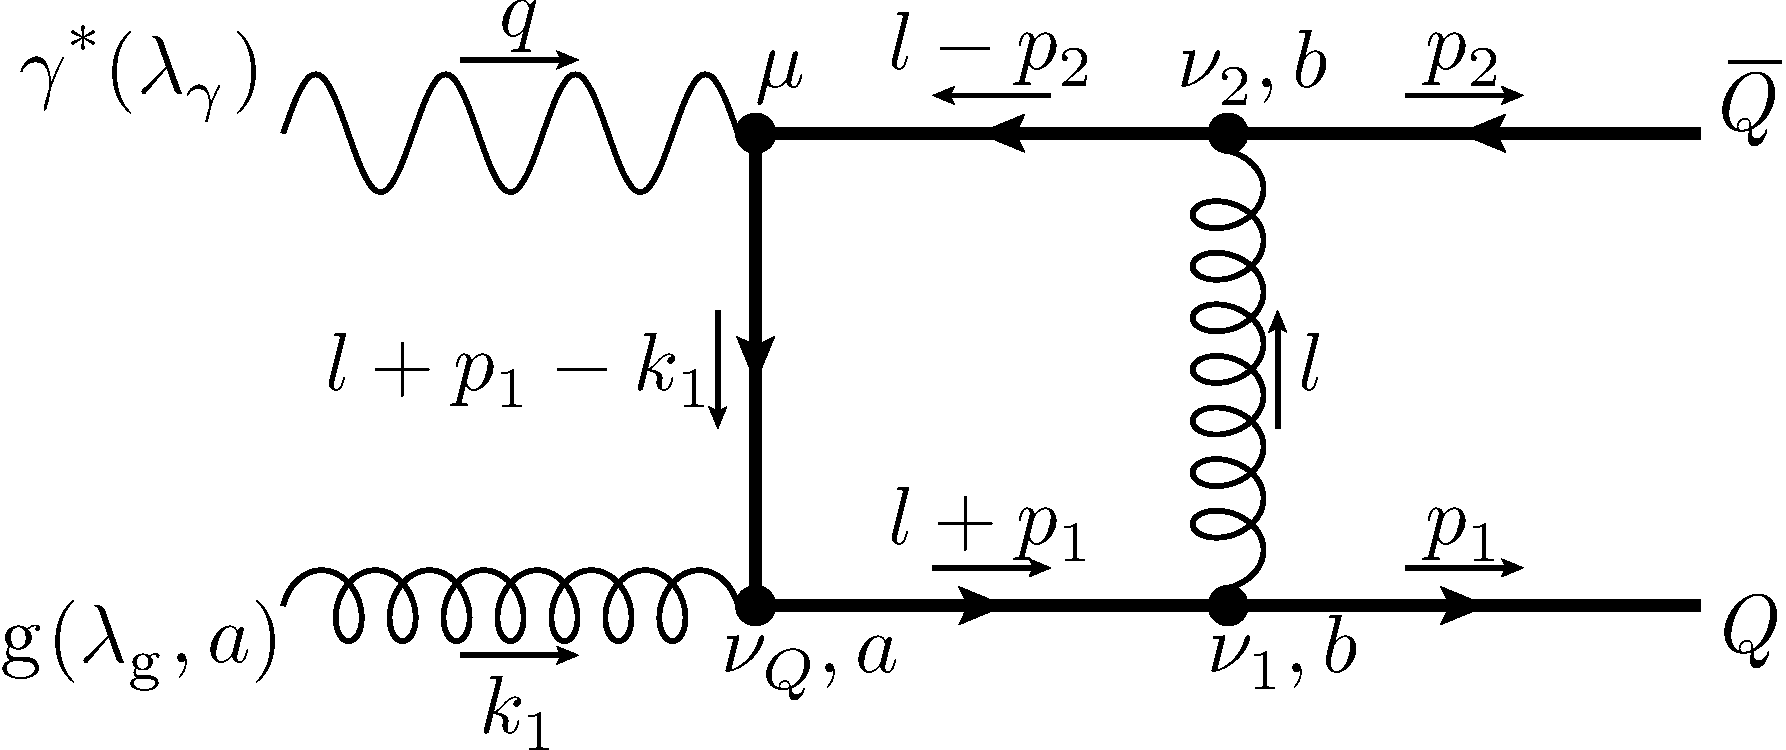
\includegraphics[width=\textwidth]{pyfeyn/nlo-v-box1}
		\caption{$i\Md^{(NLO,v)}_{1,\mu}$}
	\end{subfigure}\hspace{.15\textwidth}%
	\begin{subfigure}[t]{.4\textwidth}
		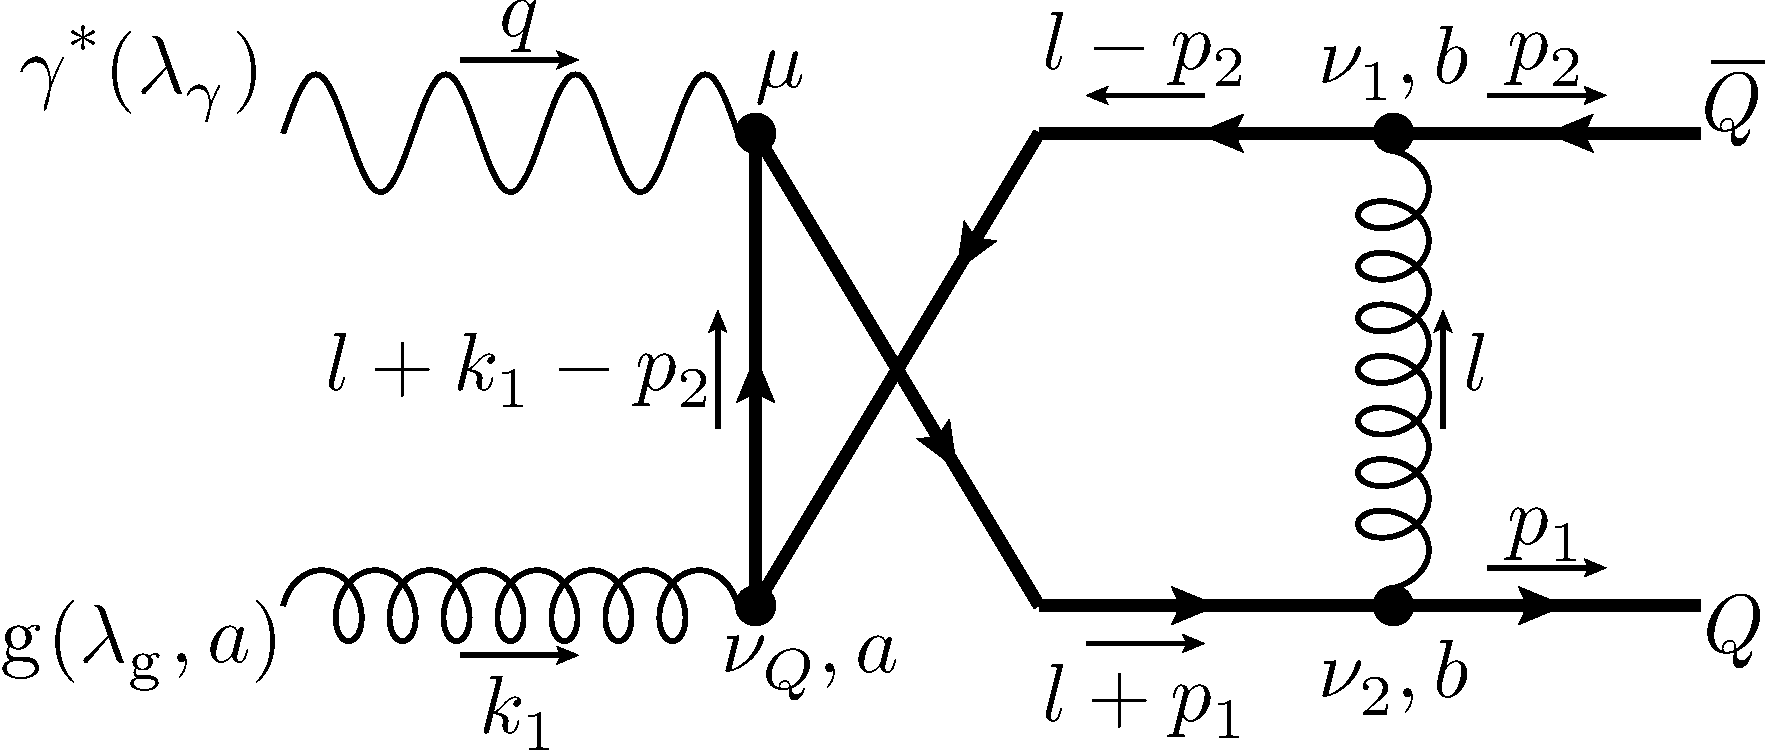
\includegraphics[width=\textwidth]{pyfeyn/nlo-v-box1cr}
		\caption{$i\Md^{(NLO,v)}_{2,\mu}$}
	\end{subfigure}\\
	\begin{subfigure}[t]{.6\textwidth}
		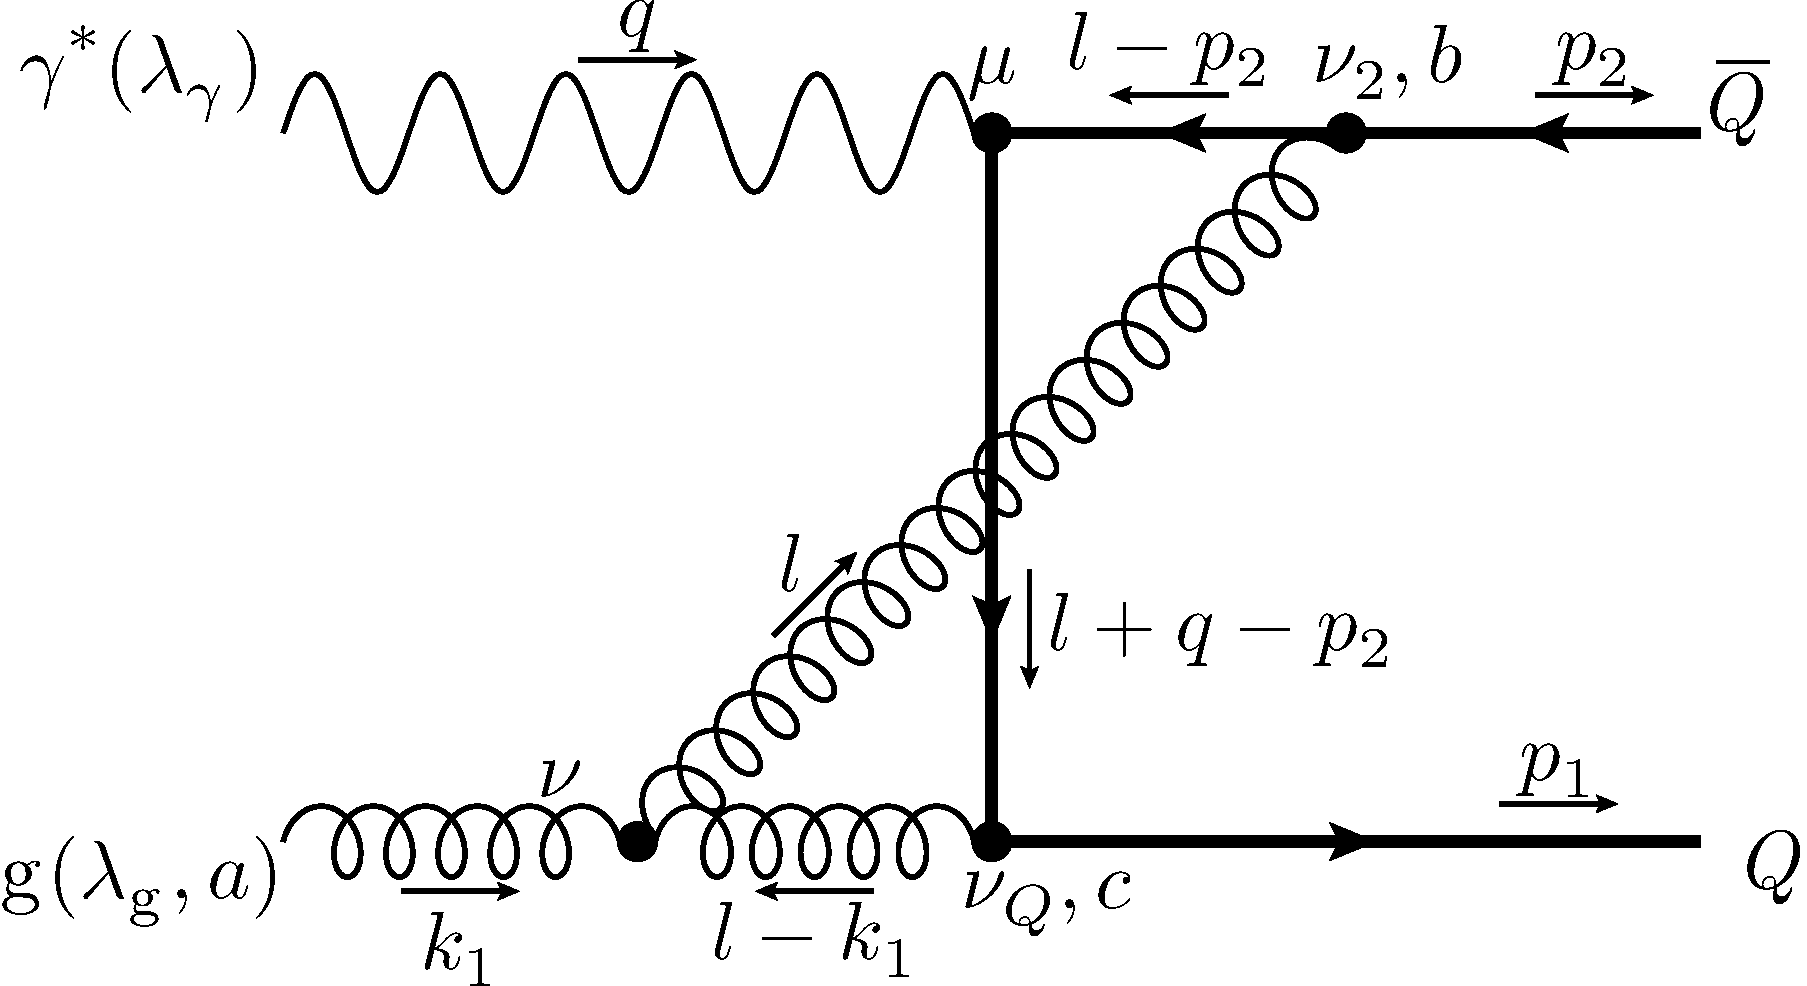
\includegraphics[width=\textwidth]{pyfeyn/nlo-v-box2}
		\caption{$i\Md^{(NLO,v)}_{3,\mu}$}
	\end{subfigure}
	\caption{NLO contributions by one loop}\label{fig:FeynNLOvab}
\end{figure}

\begin{align}
i\Md^{(NLO,v)}_{1,\mu} &=\mu_R^{4-n}\!\!\int\!\!\frac{d^nl}{(2\pi)^n}\,\bar u(p_1)(igT_b\gamma^{\nu_1})\frac{i(\slashed{l}+\slashed{p}_1+m)}{(l+p_1)^2-m^2}(igT_a\gamma^{\nu_Q})\frac{i(\slashed{l}+\slashed{p}_1-\slashed{k}_1+m)}{(l+p_1-k_1)^2-m^2}\cdot\nonumber\\
 &\hspace{40pt}(-i e e_H \gamma_\mu)\frac{i(\slashed{l}-\slashed{p}_2+m)}{(l-p_2)^2-m^2}(igT_b\gamma^{\nu_2})\frac{-ig_{\nu_1,\nu_2}}{l^2}v(p_2)\varepsilon^{(\lambda_{\Pg})}_{\nu_Q}(k_1)\\
i\Md^{(NLO,v)}_{2,\mu} &= \mu_R^{4-n}\!\!\int\!\!\frac{d^nl}{(2\pi)^n}\,\bar u(p_1)(igT_b\gamma^{\nu_1})\frac{i(\slashed{l}+\slashed{p}_1+m)}{(l+p_1)^2-m^2}(igT_a\gamma^{\nu_Q})\frac{i(\slashed{l}+\slashed{p}_1-\slashed{q}+m)}{(l+p_1-q)^2-m^2}\cdot\nonumber\\
 &\hspace{40pt}(-i e e_H \gamma_\mu)\frac{i(\slashed{l}-\slashed{p}_2+m)}{(l-p_2)^2-m^2}(igT_b\gamma^{\nu_2})\frac{-ig_{\nu_1,\nu_2}}{l^2}v(p_2)\varepsilon^{(\lambda_{\Pg})}_{\nu_Q}(k_1)\\
i\Md^{(NLO,v)}_{3,\mu} &=\mu_R^{4-n}\!\!\int\!\!\frac{d^nl}{(2\pi)^n}\,\bar u(p_1)(igT_c\gamma^{\nu_Q})\frac{i(\slashed{l}+\slashed{q}_1-\slashed{p}_2+m)}{(l+q-p_2)^2-m^2}(-i e e_H \gamma_\mu)\frac{i(\slashed{l}-\slashed{p}_2+m)}{(l-p_2)^2-m^2}\cdot\nonumber\\
 &\hspace{20pt}(igT_b\gamma^{\nu_2})\frac{(-i)^2}{l^2(l-k_1)^2}v(p_2)\varepsilon^{\nu,(\lambda_{\Pg})}(k_1)\cdot\nonumber\\
 &\hspace{20pt}\left(gf_{abc}\left(g_{\nu_2\nu_Q}(k_1-2l)_\nu+g_{\nu_Q\nu}(l-2k_1)_{\nu_2}+g_{\nu\nu_2}(k_1+l)_{\nu_Q}\right)\right)
\end{align}

\pagebreak

\begin{figure}[ht!]
	\begin{subfigure}[t]{.4\textwidth}
		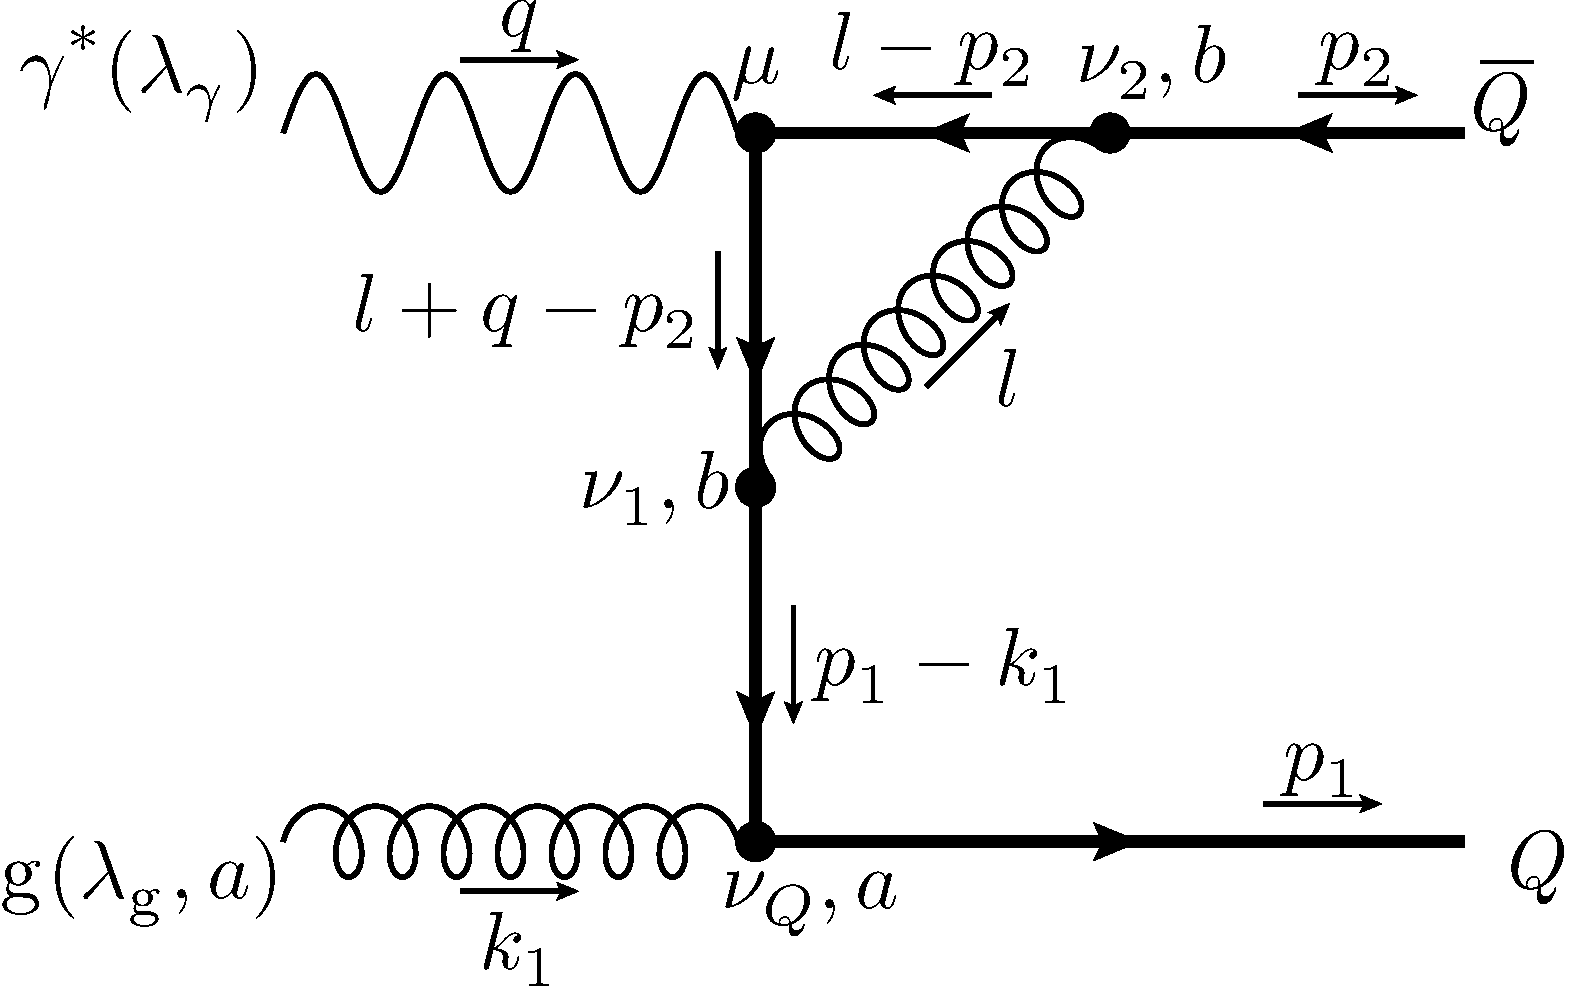
\includegraphics[width=\textwidth]{pyfeyn/nlo-v-e}
		\caption{$i\Md^{(NLO,v)}_{5,\mu}$}
	\end{subfigure}\hspace{.15\textwidth}%
	\begin{subfigure}[t]{.4\textwidth}
		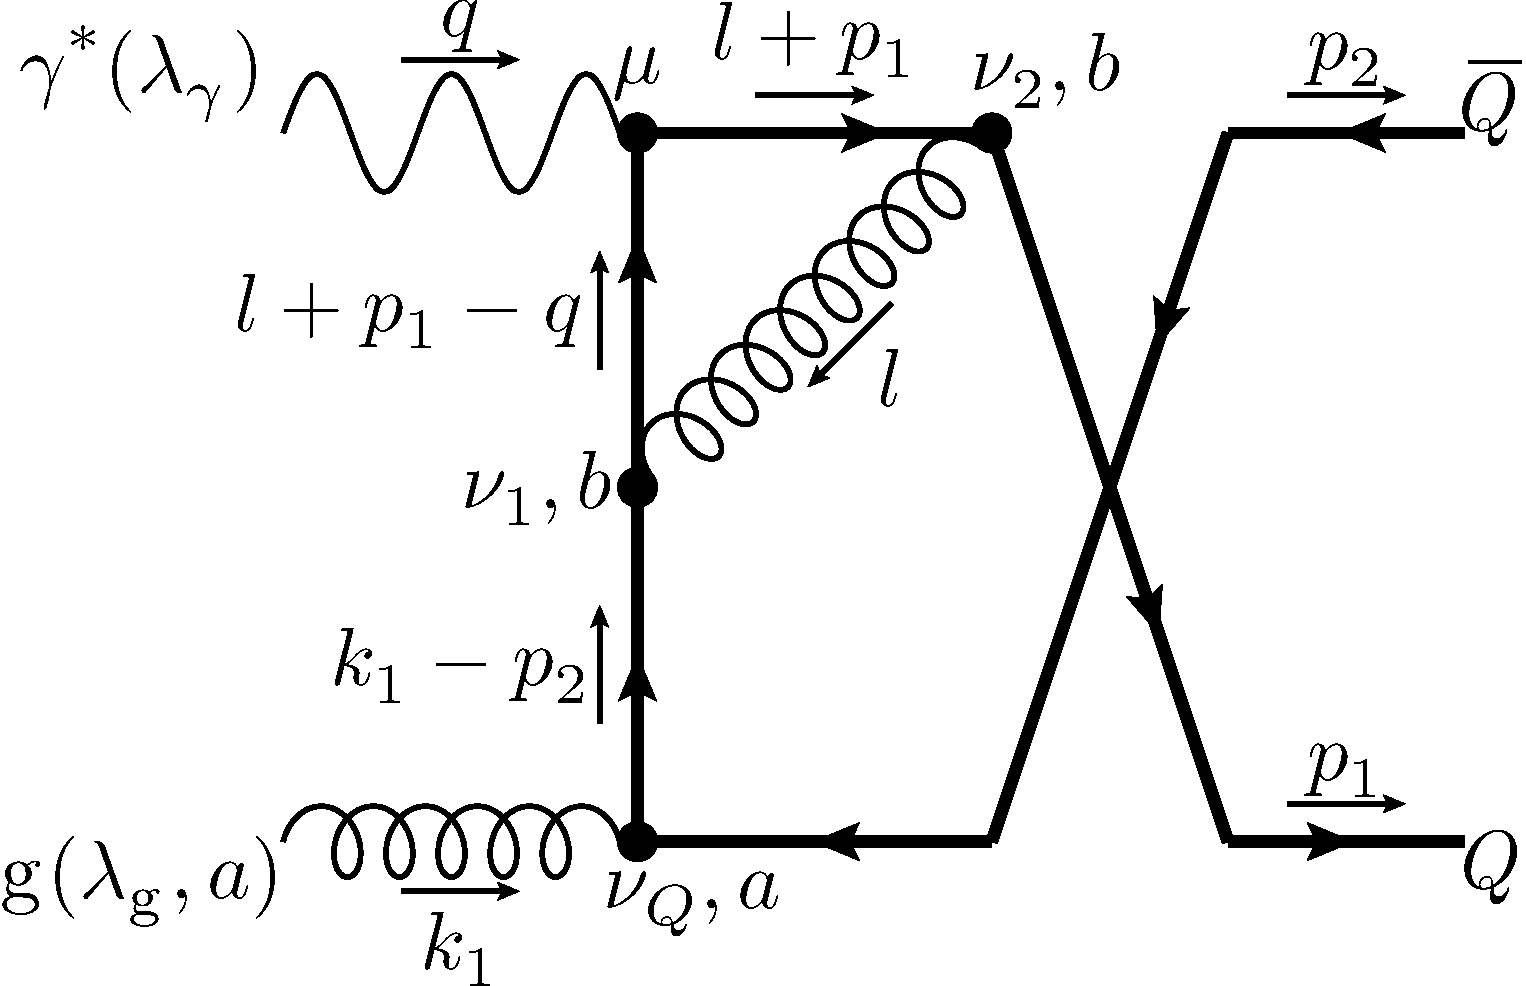
\includegraphics[width=\textwidth]{pyfeyn/nlo-v-ecr}
		\caption{$i\Md^{(NLO,v)}_{6,\mu}$}
	\end{subfigure}\\
	\begin{subfigure}[t]{.4\textwidth}
		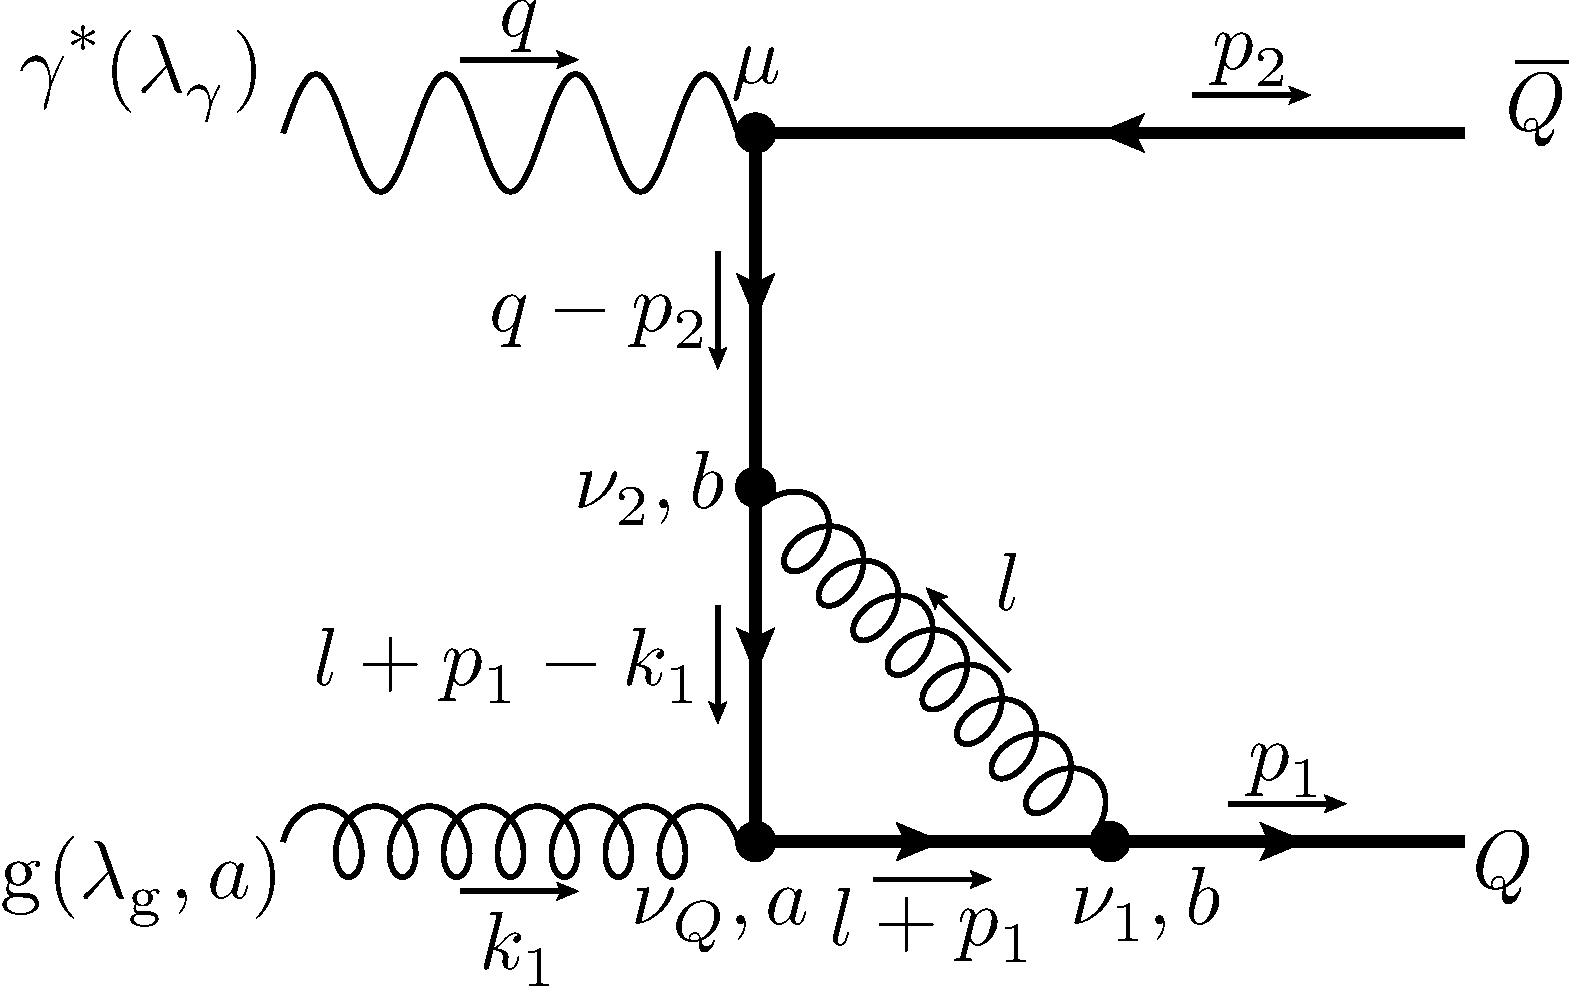
\includegraphics[width=\textwidth]{pyfeyn/nlo-v-g1}
		\caption{$i\Md^{(NLO,v)}_{7,\mu}$}
	\end{subfigure}\hspace{.15\textwidth}%
	\begin{subfigure}[t]{.4\textwidth}
		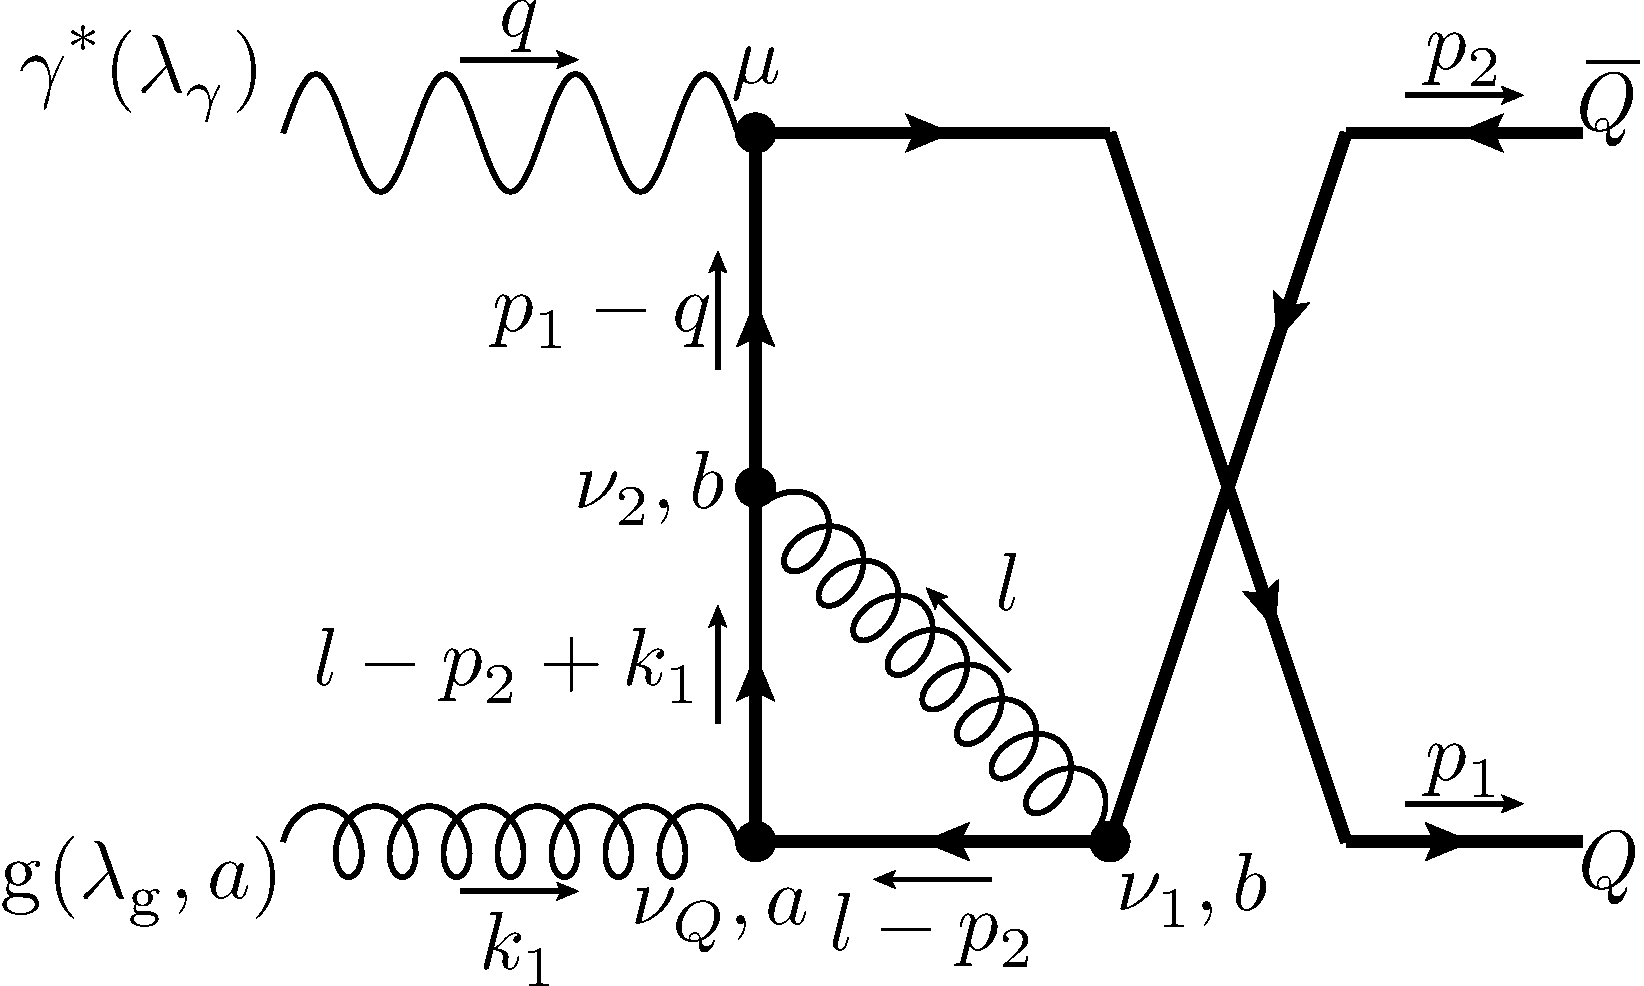
\includegraphics[width=\textwidth]{pyfeyn/nlo-v-g1cr}
		\caption{$i\Md^{(NLO,v)}_{8,\mu}$}
	\end{subfigure}
	\caption{NLO contributions by one loop (cont'ed)}\label{fig:FeynNLOvcd}
\end{figure}

\begin{align}
i\Md^{(NLO,v)}_{5,\mu} &=\mu_R^{4-n}\!\!\int\!\!\frac{d^nl}{(2\pi)^n}\,\bar u(p_1)(igT_a\gamma^{\nu_Q})\frac{i(\slashed{p}_1-\slashed{k}_1+m)}{u_1}(igT_b\gamma^{\nu_1})\frac{i(\slashed{l}+\slashed{q}-\slashed{p}_2+m)}{(l+q-p_2)^2-m^2}\cdot\nonumber\\
 &\hspace{40pt}(-i e e_H \gamma_\mu)\frac{i(\slashed{l}-\slashed{p}_2+m)}{(l-p_2)^2-m^2}(igT_b\gamma^{\nu_2})\frac{-ig_{\nu_1,\nu_2}}{l^2}v(p_2)\varepsilon^{(\lambda_{\Pg})}_{\nu_Q}(k_1)\\
i\Md^{(NLO,v)}_{6,\mu} &=\mu_R^{4-n}\!\!\int\!\!\frac{d^nl}{(2\pi)^n}\,\bar u(p_1)(igT_b\gamma^{\nu_2})\frac{i(\slashed{l}+\slashed{p}_1+m)}{(l+p_1)^2-m^2}(-i e e_H \gamma_\mu)\frac{i(\slashed{l}+\slashed{p}_1-\slashed{q}+m)}{(l+p_1-q)^2-m^2}\cdot\nonumber\\
 &\hspace{40pt}(igT_b\gamma^{\nu_1})\frac{i(\slashed{k}_1-\slashed{p}_2+m)}{t_1}(igT_a\gamma^{\nu_Q})\frac{-ig_{\nu_1,\nu_2}}{l^2}v(p_2)\varepsilon^{(\lambda_{\Pg})}_{\nu_Q}(k_1)\\
i\Md^{(NLO,v)}_{7,\mu} &=\mu_R^{4-n}\!\!\int\!\!\frac{d^nl}{(2\pi)^n}\,\bar u(p_1)(igT_b\gamma^{\nu_1})\frac{i(\slashed{l}+\slashed{p}_1+m)}{(l+p_1)^2-m^2}(igT_a\gamma^{\nu_Q})\frac{i(\slashed{l}+\slashed{p}_1-\slashed{k}_1+m)}{(l+p_1-k_1)^2-m^2}\cdot\nonumber\\
 &\hspace{40pt}(igT_b\gamma^{\nu_2})\frac{i(\slashed{q}-\slashed{p}_2+m)}{u_1}(-i e e_H \gamma_\mu)\frac{-ig_{\nu_1,\nu_2}}{l^2}v(p_2)\varepsilon^{(\lambda_{\Pg})}_{\nu_Q}(k_1)\\
i\Md^{(NLO,v)}_{8,\mu} &=\mu_R^{4-n}\!\!\int\!\!\frac{d^nl}{(2\pi)^n}\,\bar u(p_1)(-i e e_H \gamma_\mu)\frac{i(\slashed{p}_1-\slashed{q}+m)}{t_1}(igT_b\gamma^{\nu_2})\frac{i(\slashed{l}-\slashed{p}_2+\slashed{k}_1+m)}{(l-p_2+k_1)^2-m^2}\cdot\nonumber\\
 &\hspace{40pt}(igT_a\gamma^{\nu_Q})\frac{i(\slashed{l}-\slashed{p}_2+m)}{(l-p_2)^2-m^2}(igT_b\gamma^{\nu_1})\frac{-ig_{\nu_1,\nu_2}}{l^2}v(p_2)\varepsilon^{(\lambda_{\Pg})}_{\nu_Q}(k_1)
\end{align}

\pagebreak

\begin{figure}[ht!]
	\begin{subfigure}[t]{.4\textwidth}
		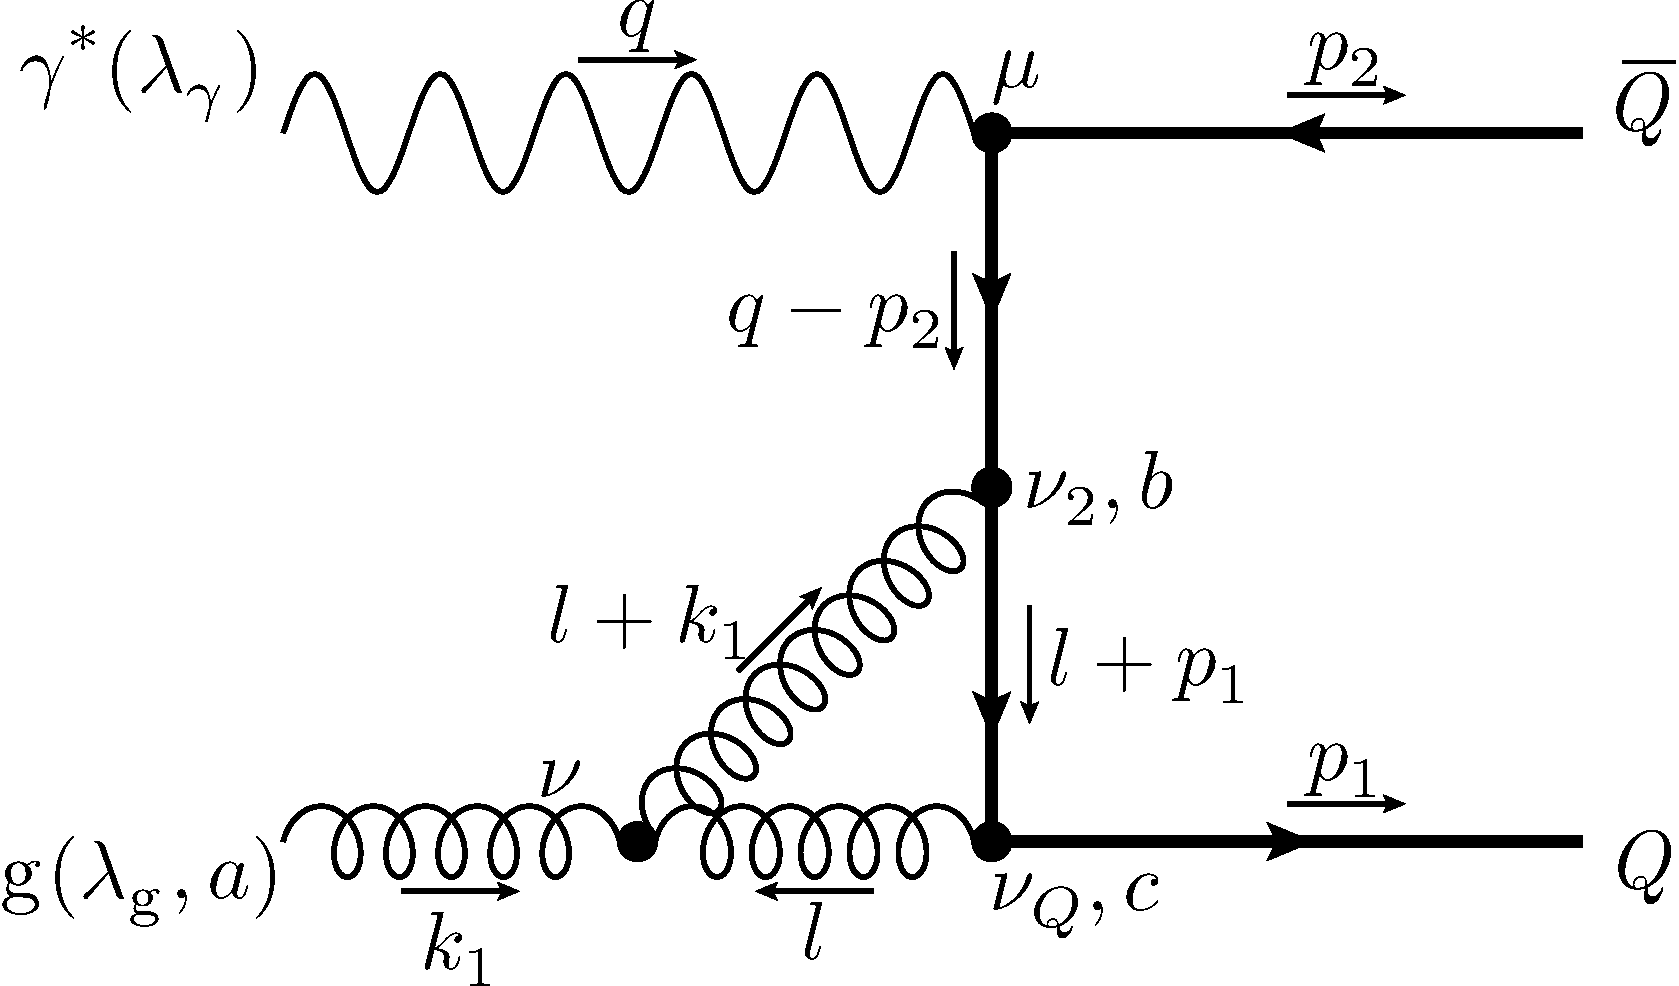
\includegraphics[width=\textwidth]{pyfeyn/nlo-v-g2}
		\caption{$i\Md^{(NLO,v)}_{9,\mu}$}
	\end{subfigure}\hspace{.15\textwidth}%
	\begin{subfigure}[t]{.4\textwidth}
		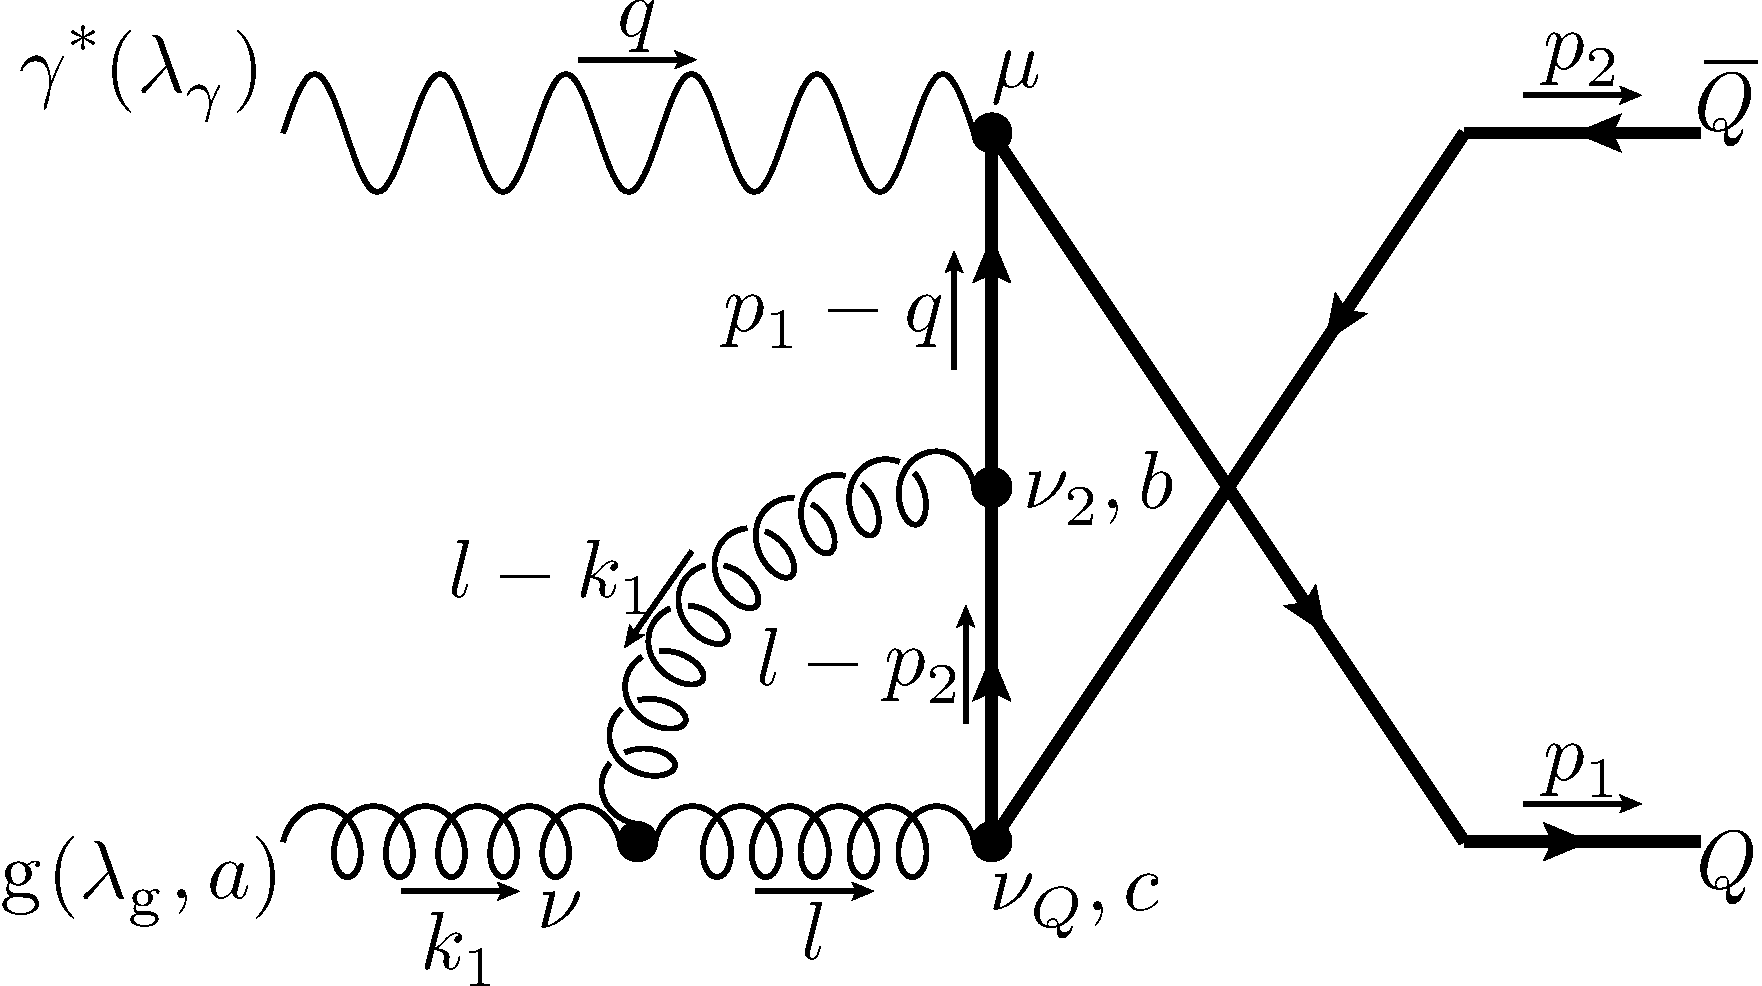
\includegraphics[width=\textwidth]{pyfeyn/nlo-v-g2cr}
		\caption{$i\Md^{(NLO,v)}_{10,\mu}$}
	\end{subfigure}\\
	\begin{subfigure}[t]{.4\textwidth}
		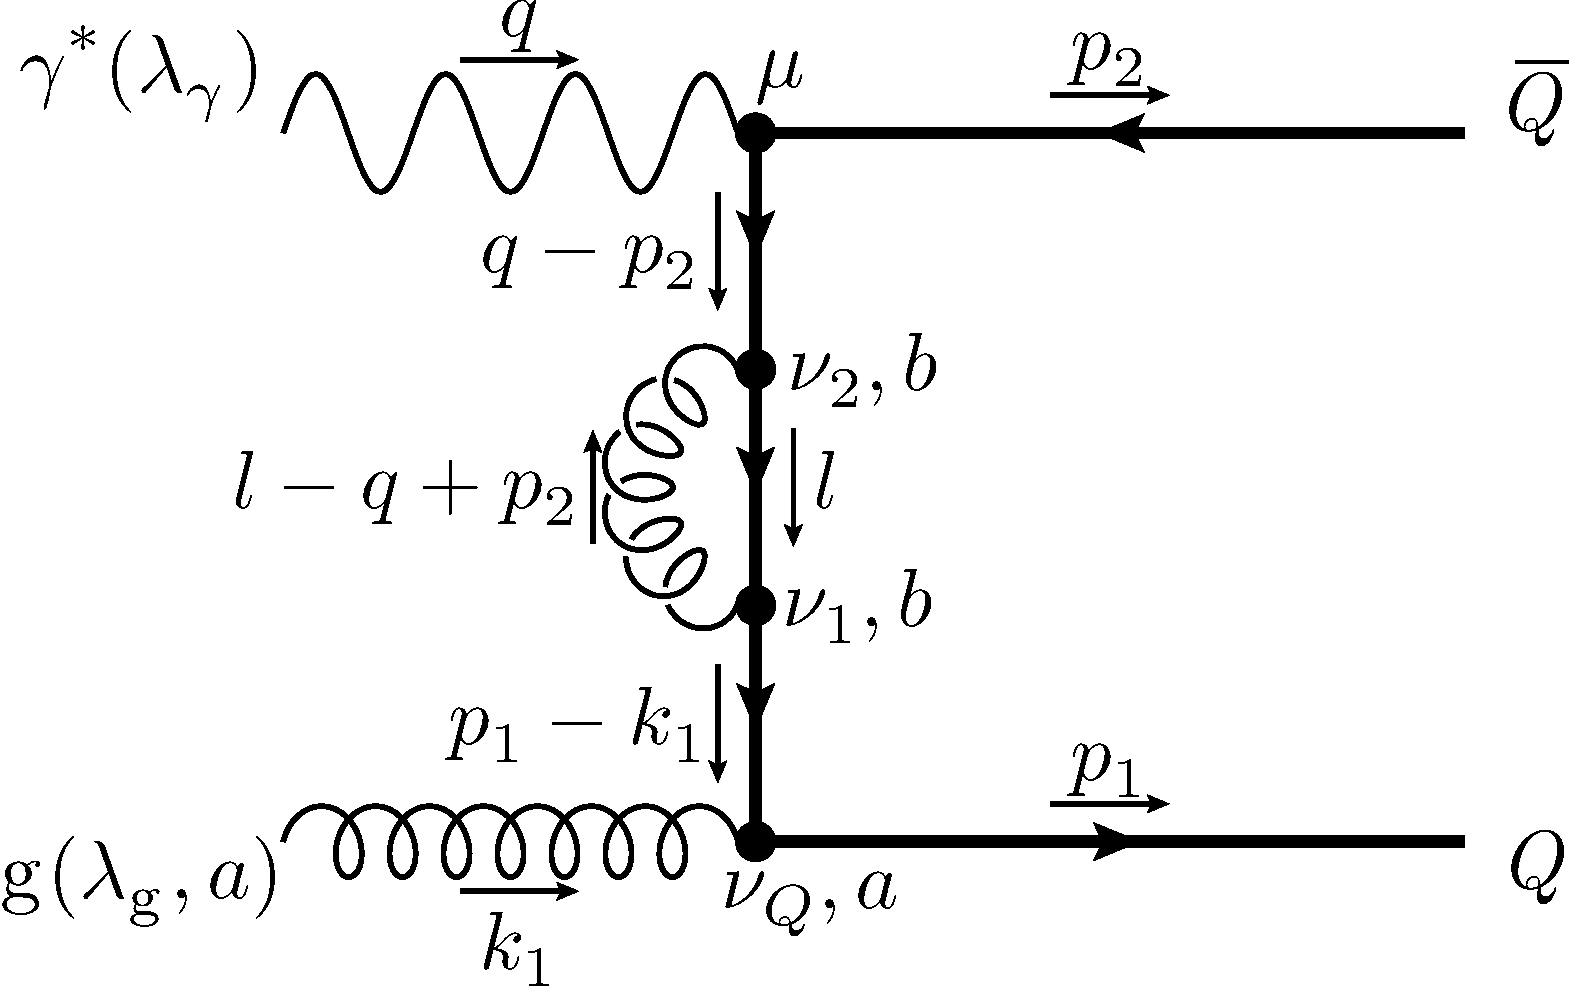
\includegraphics[width=\textwidth]{pyfeyn/nlo-v-m1}
		\caption{$i\Md^{(NLO,v)}_{11,\mu}$}
	\end{subfigure}\hspace{.15\textwidth}%
	\begin{subfigure}[t]{.4\textwidth}
		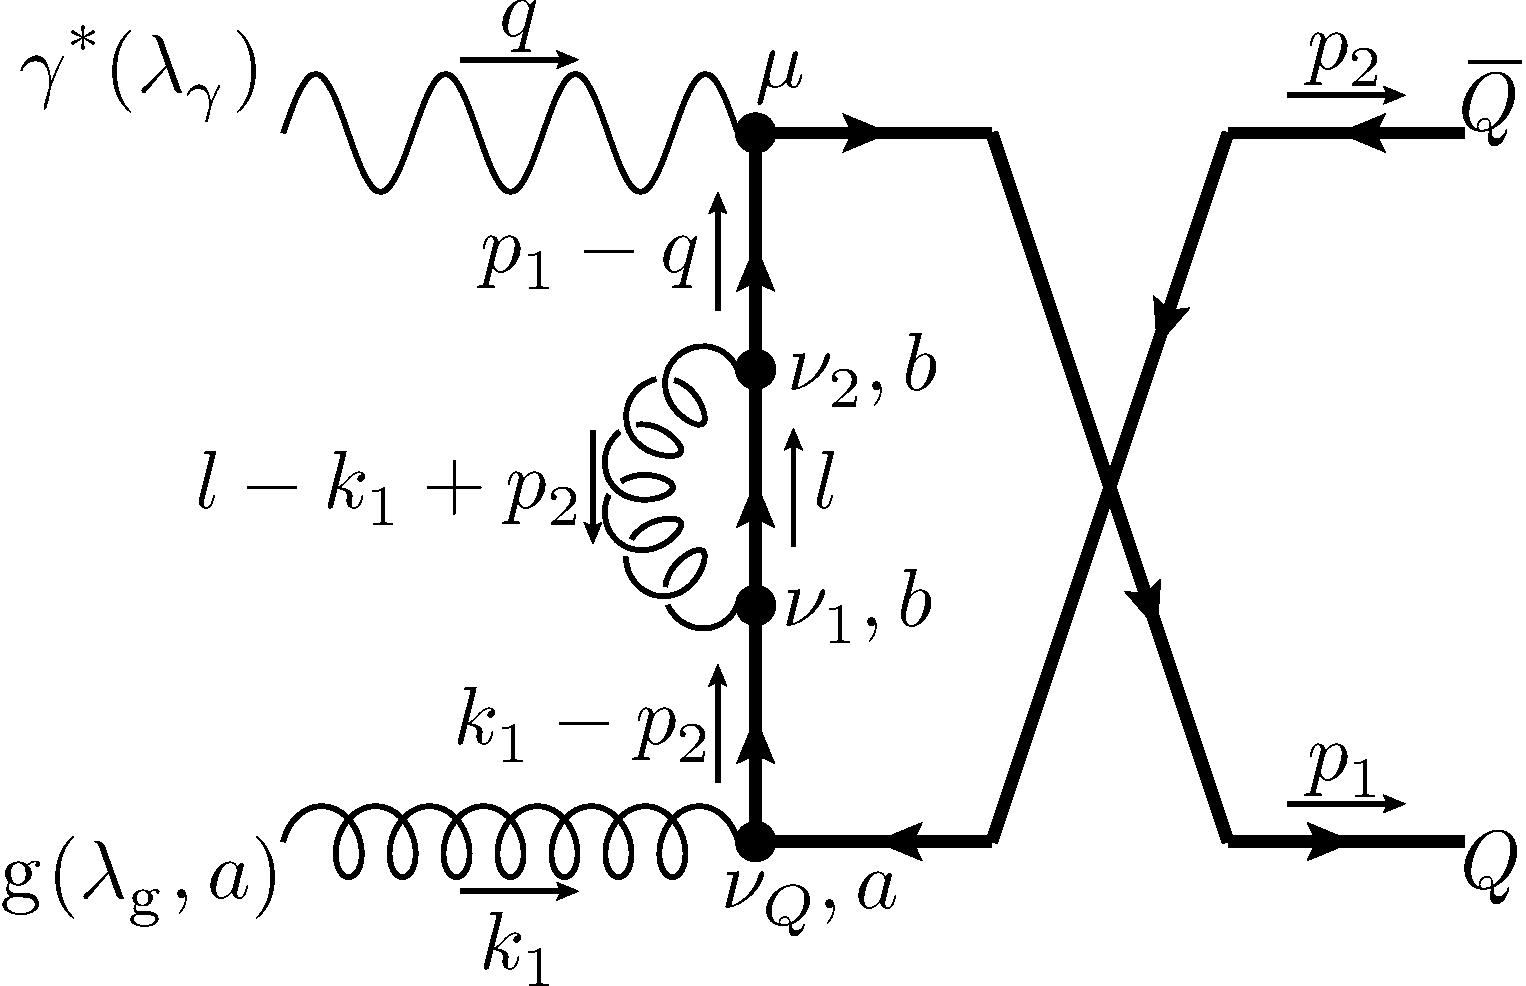
\includegraphics[width=\textwidth]{pyfeyn/nlo-v-m1cr}
		\caption{$i\Md^{(NLO,v)}_{12,\mu}$}
	\end{subfigure}
	\caption{NLO contributions by one loop (cont'ed)}\label{fig:FeynNLOve}
\end{figure}

\begin{align}
i\Md^{(NLO,v)}_{9,\mu} &=\mu_R^{4-n}\!\!\int\!\!\frac{d^nl}{(2\pi)^n}\,\bar u(p_1)(igT_c\gamma^{\nu_Q})\frac{i(\slashed{l}+\slashed{p}_1+m)}{(l+p_1)^2-m^2}(igT_b\gamma^{\nu_2})\frac{i(\slashed{q}-\slashed{p}_2+m)}{u_1}\cdot\nonumber\\
 &\hspace{20pt}(-i e e_H \gamma_\mu)\frac{(-i)^2}{l^2(l+k_1)^2}v(p_2)\varepsilon^{\nu,(\lambda_{\Pg})}(k_1)\cdot\nonumber\\
 &\hspace{20pt}\left(gf_{abc}\left(g_{\nu\nu_2}(2k_1+l)_{\nu_Q}+g_{\nu_2\nu_Q}(-2l-k_1)_{\nu}+g_{\nu_Q\nu}(l-k_1)_{\nu_2}\right)\right)\\
i\Md^{(NLO,v)}_{10,\mu} &=\mu_R^{4-n}\!\!\int\!\!\frac{d^nl}{(2\pi)^n}\,\bar u(p_1)(-i e e_H \gamma_\mu)\frac{i(\slashed{p}_1-\slashed{q}+m)}{t_1}(igT_b\gamma^{\nu_2})\frac{i(\slashed{l}-\slashed{p}_2+m)}{(l-p_2)^2-m^2}\cdot\nonumber\\
 &\hspace{20pt}(igT_c\gamma^{\nu_Q})\frac{(-i)^2}{l^2(l-k_1)^2}v(p_2)\varepsilon^{\nu,(\lambda_{\Pg})}(k_1)\cdot\nonumber\\
 &\hspace{20pt}\left(gf_{abc}\left(g_{\nu\nu_2}(2k_1-l)_{\nu_Q}+g_{\nu_2\nu_Q}(2l-k_1)_{\nu}+g_{\nu_Q\nu}(-l-k_1)_{\nu_2}\right)\right)\\
i\Md^{(NLO,v)}_{11,\mu} &=\mu_R^{4-n}\!\!\int\!\!\frac{d^nl}{(2\pi)^n}\,\bar u(p_1)(igT_a\gamma^{\nu_Q})\frac{i(\slashed{p}_1-\slashed{k}_1+m)}{u_1}(igT_b\gamma^{\nu_1})\frac{i(\slashed{l}+m)}{l^2-m^2}\cdot\nonumber\\
 &\hspace{40pt}(igT_b\gamma^{\nu_2})\frac{i(\slashed{q}-\slashed{p}_2+m)}{u_1}(-i e e_H \gamma_\mu)\frac{-ig_{\nu_1,\nu_2}}{(l-q+p_2)^2}v(p_2)\varepsilon^{(\lambda_{\Pg})}_{\nu_Q}(k_1)\\
i\Md^{(NLO,v)}_{12,\mu} &=\mu^{4-n}\!\!\int\!\!\frac{d^nl}{(2\pi)^n}\,\bar u(p_1)(-i e e_H \gamma_\mu)\frac{i(\slashed{p}_1-\slashed{q}+m)}{t_1}(igT_b\gamma^{\nu_2})\frac{i(\slashed{l}+m)}{l^2-m^2}\cdot\nonumber\\
 &\hspace{40pt}(igT_b\gamma^{\nu_1})\frac{i(\slashed{k}_1-\slashed{p}_2+m)}{t_1}(igT_a\gamma^{\nu_Q})\frac{-ig_{\nu_1,\nu_2}}{(l-k_1+p_2)^2}v(p_2)\varepsilon^{(\lambda_{\Pg})}_{\nu_Q}(k_1)
\end{align}

Color space:
\begin{align}
&\left(\Md^{(NLO,v)}_{1,\mu}+\Md^{(NLO,v)}_{2,\mu} + \Md^{(NLO,v)}_{7,\mu}+\Md^{(NLO,v)}_{8,\mu}\right)\nonumber\\
&\hspace{20pt}\cdot\left(\Md^{(LO)}_{1,\mu'}+\Md^{(LO)}_{2,\mu'}\right)^*\sim -i\tr(T_aT_bT_aT_b) = -iN_C C_F \left(C_F - \frac{C_A}{2}\right)\\
&\left(\Md^{(NLO,v)}_{3,\mu}+ \Md^{(NLO,v)}_{9,\mu}+\Md^{(NLO,v)}_{10,\mu}\right)\nonumber\\
&\hspace{20pt}\cdot\left(\Md^{(LO)}_{1,\mu'}+\Md^{(LO)}_{2,\mu'}\right)^*\sim f_{abc}\tr(T_cT_bT_a) = -\frac i 2 N_C C_F C_A\\
&\left(\Md^{(NLO,v)}_{5,\mu}+\Md^{(NLO,v)}_{6,\mu}+\Md^{(NLO,v)}_{11,\mu}+\Md^{(NLO,v)}_{12,\mu}\right)\nonumber\\
&\hspace{20pt}\cdot\left(\Md^{(LO)}_{1,\mu'}+\Md^{(LO)}_{2,\mu'}\right)^*\sim -i\tr(T_aT_aT_bT_b) = -iN_C C_F^2
\end{align}


\subsubsection{Counter terms}
\begin{figure}[ht!]
	\begin{subfigure}[t]{.4\textwidth}
		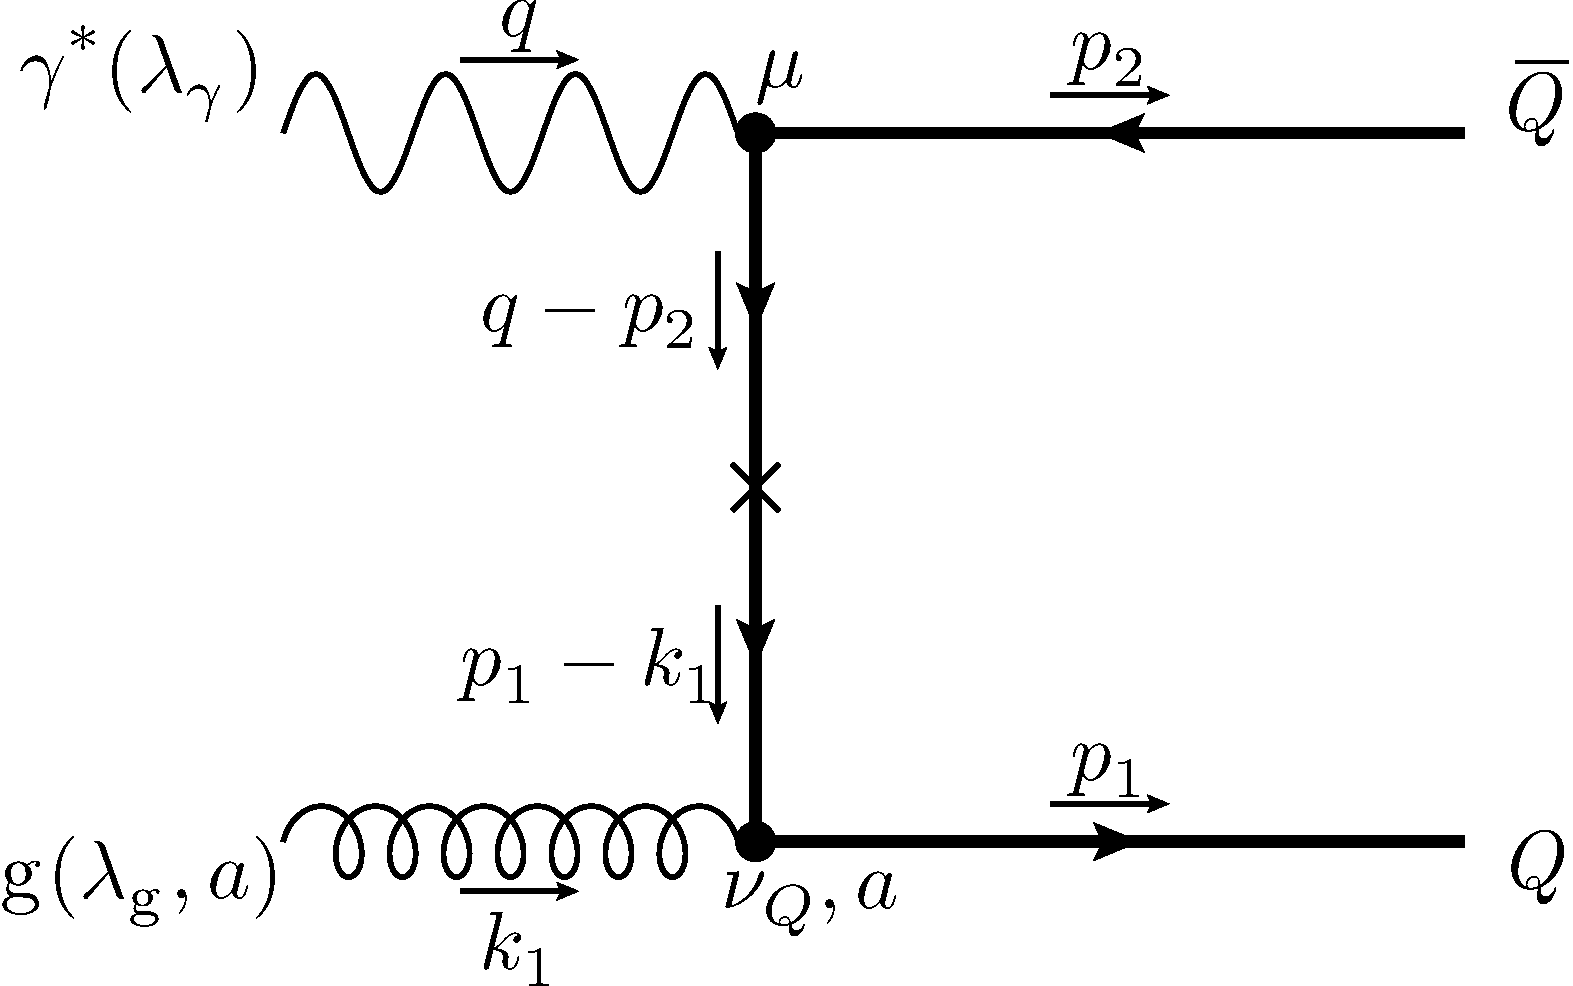
\includegraphics[width=\textwidth]{pyfeyn/nlo-c-m}
		\caption{$i\Md^{(NLO,c)}_{1,\mu}$}
	\end{subfigure}\hspace{.15\textwidth}%
	\begin{subfigure}[t]{.4\textwidth}
		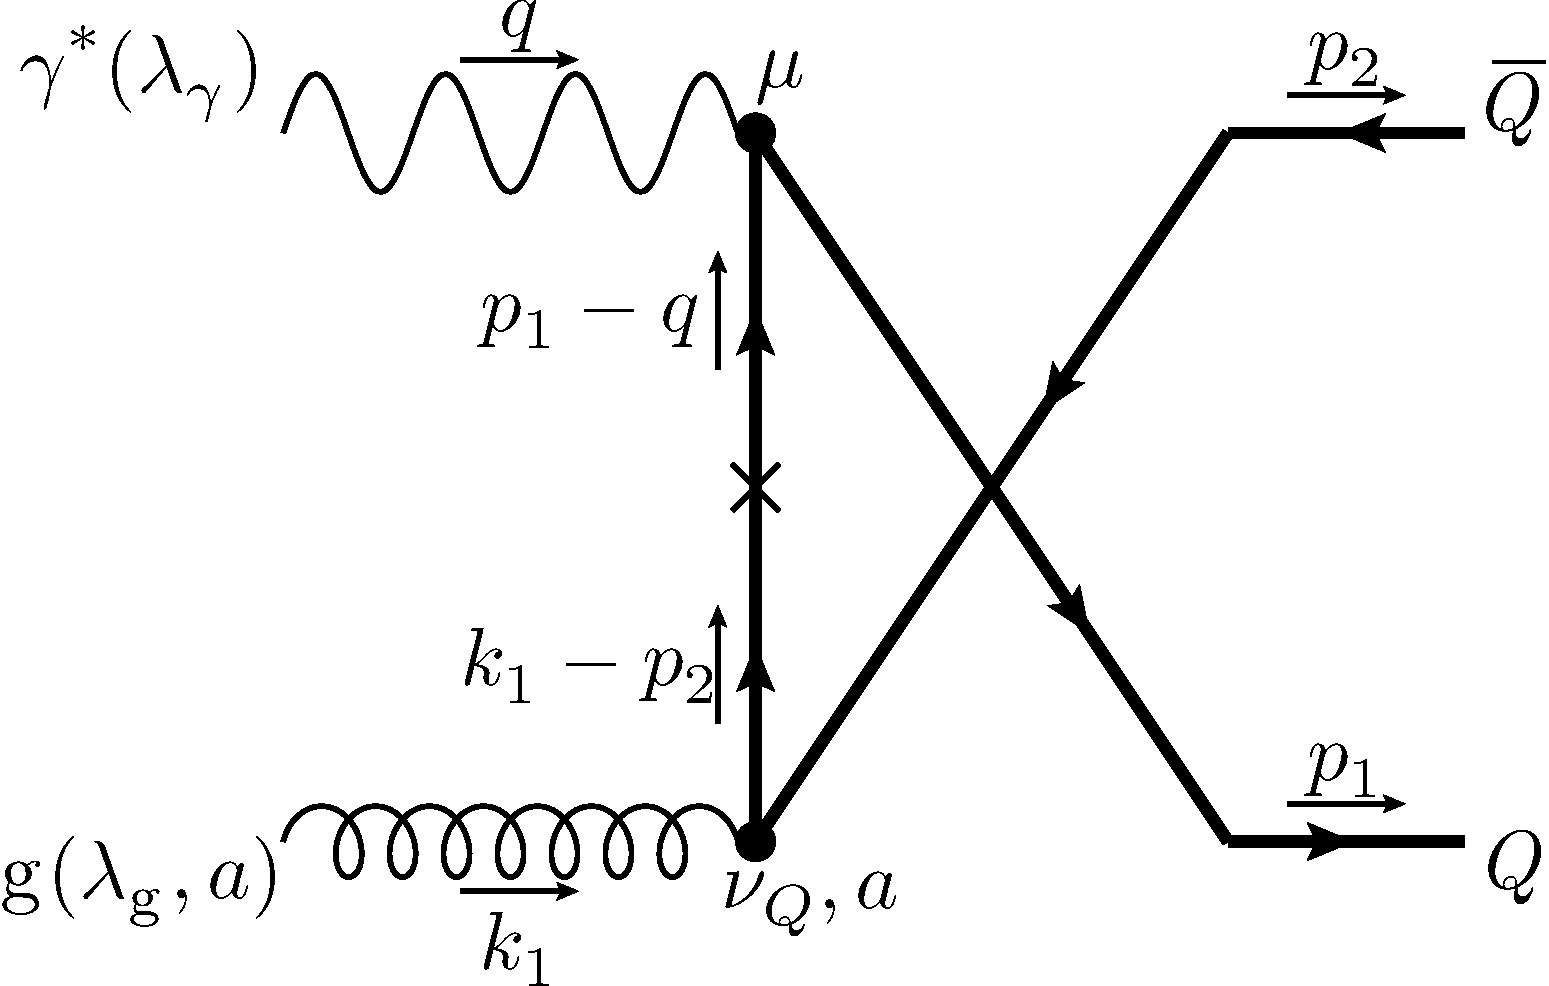
\includegraphics[width=\textwidth]{pyfeyn/nlo-c-mcr}
		\caption{$i\Md^{(NLO,c)}_{2,\mu}$}
	\end{subfigure}\\
	\begin{subfigure}[t]{.4\textwidth}
		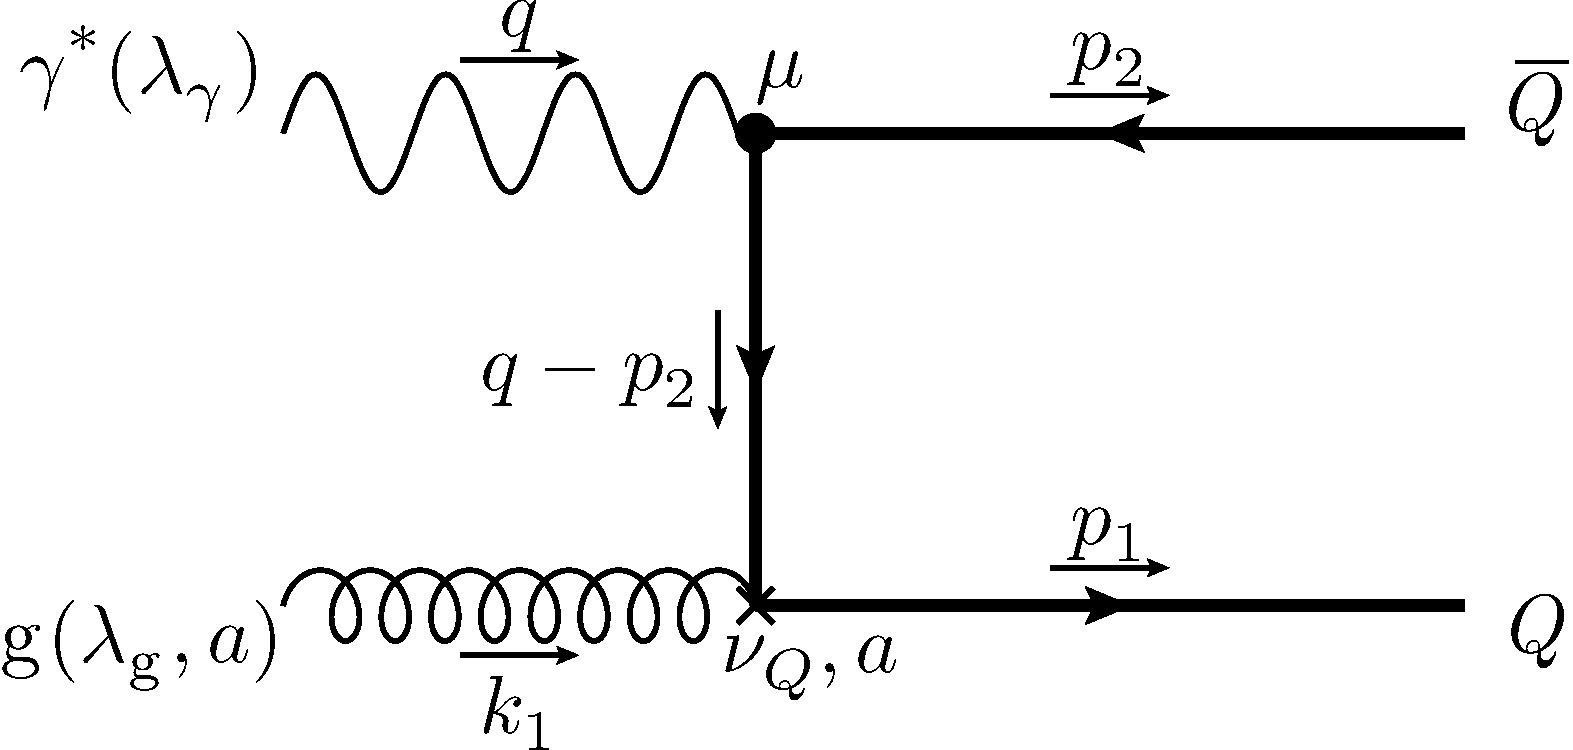
\includegraphics[width=\textwidth]{pyfeyn/nlo-c-nuQ}
		\caption{$i\Md^{(NLO,c)}_{3,\mu}$}
	\end{subfigure}\hspace{.15\textwidth}%
	\begin{subfigure}[t]{.4\textwidth}
		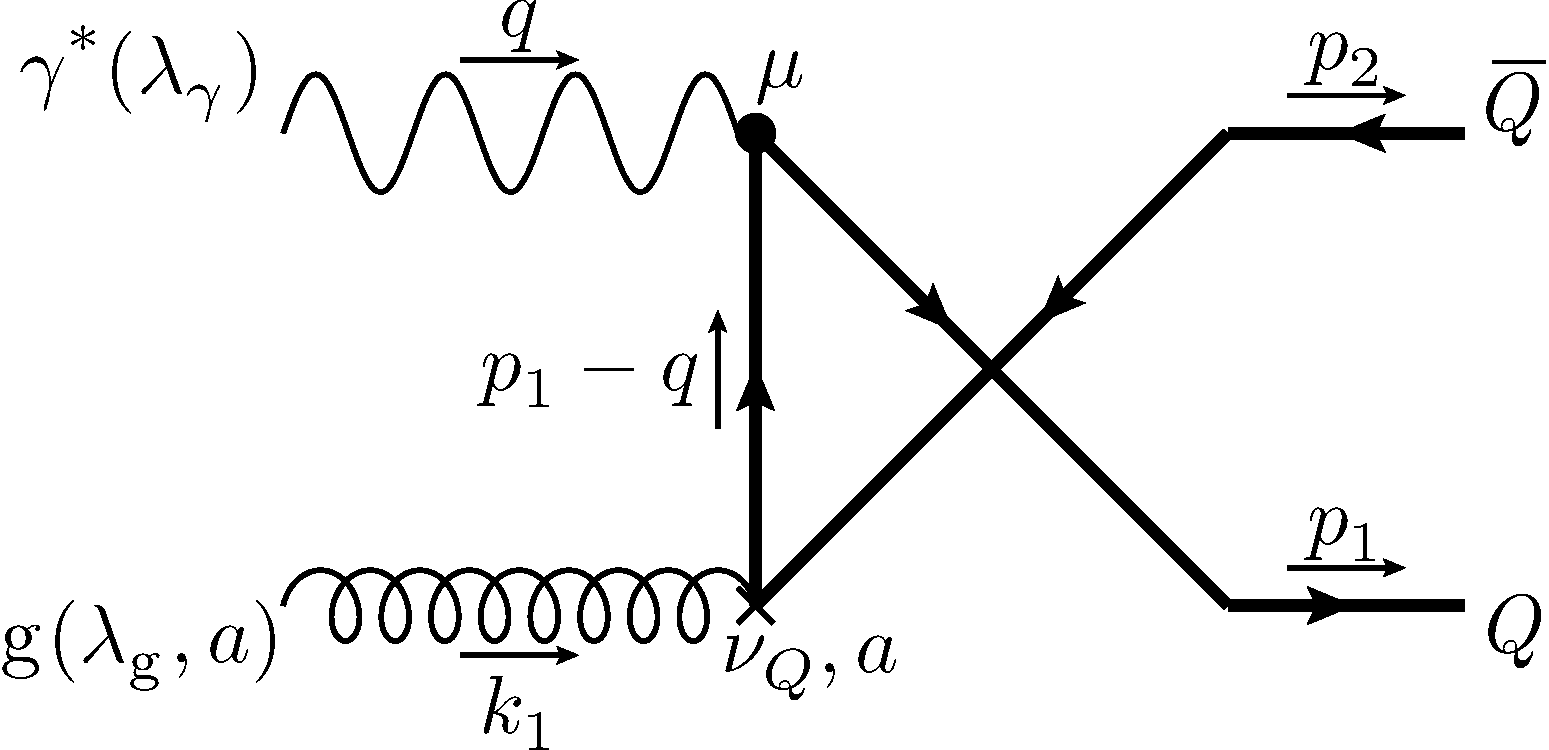
\includegraphics[width=\textwidth]{pyfeyn/nlo-c-nuQcr}
		\caption{$i\Md^{(NLO,c)}_{4,\mu}$}
	\end{subfigure}
	\caption{NLO contributions by counter terms}\label{fig:FeynNLOvf}
\end{figure}

\begin{align}
-i\Md^{(NLO,c)}_{1,\mu} &=\bar u(p_1)(igT_a\gamma^{\nu_Q})\frac{i(\slashed{p}_1-\slashed{k}_1+m)}{u_1}\left(i((Z_2-1)(\slashed{q} - \slashed{p}_2- m) - (Z_m-1)m)\right)\nonumber\\
&\hspace{40pt}\frac{i(\slashed{q}-\slashed{p}_2+m)}{u_1}(-i e e_H \gamma_\mu)v(p_2)\varepsilon^{(\lambda_{\Pg})}_{\nu_Q}(k_1)\\
-i\Md^{(NLO,c)}_{2,\mu} &=\bar u(p_1)(-i e e_H \gamma_\mu)\frac{i(\slashed{p}_1-\slashed{q}+m)}{t_1}\left(i((Z_2-1)(\slashed{p}_1 - \slashed{q}- m) - (Z_m-1)m)\right)\nonumber\\
&\hspace{40pt}\frac{i(\slashed{k}_1-\slashed{p}_2+m)}{t_1}(igT_a\gamma^{\nu_Q})v(p_2)\varepsilon^{(\lambda_{\Pg})}_{\nu_Q}(k_1)\\
-i\Md^{(NLO,c)}_{3,\mu} &=\bar u(p_1)(-i(Z_{1f}-1)gT_a\gamma^{\nu_Q})\frac{i(\slashed{q}-\slashed{p}_2+m)}{u_1}(-i e e_H \gamma_\mu)v(p_2)\varepsilon^{(\lambda_{\Pg})}_{\nu_Q}(k_1)\\
-i\Md^{(NLO,c)}_{4,\mu} &=\bar u(p_1)(-i e e_H \gamma_\mu)\frac{i(\slashed{p}_1-\slashed{q}+m)}{t_1}(-i(Z_{1f}-1)gT_a\gamma^{\nu_Q})v(p_2)\varepsilon^{(\lambda_{\Pg})}_{\nu_Q}(k_1)
\end{align}

Color space:
\begin{align}
\left(\Md^{(NLO,c)}_{1,\mu}+\Md^{(NLO,c)}_{2,\mu}\right)\left(\Md^{(LO)}_{1,\mu'}+\Md^{(LO)}_{2,\mu'}\right)^*&\sim \tr(T_aT_a)(Z_2-1)=N_C C_F^2\\
\left(\Md^{(NLO,c)}_{3,\mu}+\Md^{(NLO,c)}_{4,\mu}\right)\left(\Md^{(LO)}_{1,\mu'}+\Md^{(LO)}_{2,\mu'}\right)^*&\sim \tr(T_aT_a)(Z_{1f}-1)=N_C C_F(C_F+C_A)
\end{align}


\subsubsection{Quark Self Energy}
To compute self energies, we follow \cite{Bojak:2000eu}.
It is
\begin{align}
\{\gamma_\mu,\gamma_\nu\} &= 2g_{\mu\nu}\\
\gamma_\mu\gamma^\mu &= g_\mu^\mu = n \\
\gamma_\mu\gamma_\nu\gamma^\mu &= (2-n)\gamma_\nu
\end{align}
\begin{figure}[ht!]
	\begin{subfigure}[t]{.4\textwidth}
		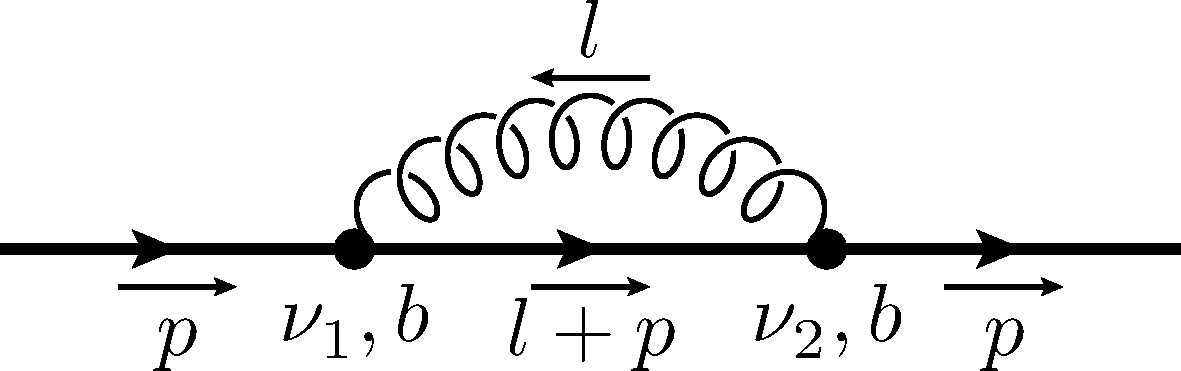
\includegraphics[width=\textwidth]{pyfeyn/nlo-v-seq}
		\caption{$-i\Sigma(p)$}
	\end{subfigure}\hspace{.15\textwidth}%
	\begin{subfigure}[t]{.4\textwidth}
		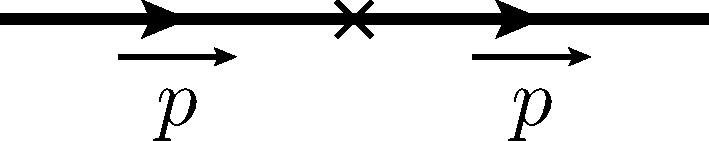
\includegraphics[width=\textwidth]{pyfeyn/nlo-v-seqc}
		\caption{$-i\Sigma_C(p)$}
	\end{subfigure}
	\caption{NLO contributions by quark self energy}\label{fig:FeynNLOvseq}
\end{figure}
\begin{align}
-i\Sigma(p) &= \mu_D^{4-n}\!\!\int\!\!\frac{d^nl}{(2\pi)^n}(igT_b \gamma_{\nu_1})\frac{i(\slashed{l}+\slashed{p}+m)}{(l+p)^2-m^2}(igT_b \gamma_{\nu_2})\frac{-ig^{\nu_1,\nu_2}}{l^2}\\
 &=-\mu_D^{4-n}g^2C_F\!\!\int\!\!\frac{d^nl}{(2\pi)^n}\frac{n\cdot m+(2-n)\slashed{p}+(2-n)\slashed{l}}{l^2((l+p)^2-m^2)}\\
 &=-g^2C_F\left(\left(n\cdot m+(2-n)\slashed{p}\right)B_0(p^2,0,m^2)+(2-n)\slashed{p}B_1(p^2,0,m^2)\right)\\
 &=-g^2C_F\left(B_0(p^2,0,m^2)\left(n\cdot m+(2-n)\slashed{p}\frac{p^2+m^2}{2p^2}\right)-(2-n)\slashed{p}\frac 1{2p^2}A_0(m^2)\right)
\end{align}
Using \cite{Bojak:2000eu} we find
\begin{align}
C_\epsilon &= \frac 1 {16\pi^2}\exp\left(\left(\gamma_E-\log(4\pi)\right)\frac{\epsilon} 2\right)\left(m^2/\mu_D^2\right)^{\epsilon/2}\\
A_0(m^2) &=iC_\epsilon\left(-\frac 2 {\epsilon}+1\right)\\
B_0(p^2,0,m^2) &=iC_\epsilon\left(-\frac 2{\epsilon}+2+\frac{m^2-p^2}{p^2}\ln\left(\frac{m^2-p^2}{m^2}\right)\right)
\end{align}
\begin{align}
\Rightarrow-i\Sigma(p) &= -ig^2C_FC_\epsilon\left[\frac{2\slashed{p}-8m}{\epsilon}+2m\left(3-2\left(1-\frac{m^2}{p^2}\right)\ln\left(1-\frac{p^2}{m^2}\right)\right)\right.\nonumber\\
 &\hspace{90pt}\left.-\slashed{p}\left(1+\frac{m^2}{p^2}\right)\left(1-\left(1-\frac{m^2}{p^2}\right)\ln\left(1-\frac{p^2}{m^2}\right)\right)\right]\\
 &\EqualClaim -i(A m + B(\slashed p - m))
\end{align}
\begin{align}
\Rightarrow A &= \frac 1 m \left.\Sigma(p)\right|_{\slashed{p}=m} \\
 &= -g^2C_F C_\epsilon\left(\frac 6 \epsilon -5 +\frac{m^2}{p^2}+\left(3-4\frac{m^2}{p^2}+\frac{m^4}{p^4}\right)\ln\left(1-\frac{p^2}{m^2}\right)\right)\\
\Rightarrow B &= \frac 1 m \left.\DeriveF{\slashed{p}}{\Sigma(p)}\right|_{\slashed{p}=m} \\
 &= \frac{g^2}{16\pi^2}C_F \left(\frac 2 {\hat\epsilon_m} -1-\frac{m^2}{p^2}+\left(1-\frac{m^4}{p^4}\right)\ln\left(1-\frac{p^2}{m^2}\right)\right)
\end{align}

Counterterm:
\begin{align}
-i\Sigma_C(p) &=i((Z_2-1)\slashed{p}-(Z_2 Z_m -1) m)\\
 &= i((Z_2-1)(\slashed p - m) - (Z_m-1)m) + O(\alpha_S^2)
\end{align}

Use on-shell renormalization:
\begin{align}
0 &\EqualClaim \left.\left(-i\Sigma(p)-i\Sigma_C(p)\right)\right|_{\slashed{p}=m}\\
 &= i\left.\left(((Z_m-1)+A)m+(B-(Z_2-1))(\slashed p - m)\right)\right|_{\slashed{p}=m} \\
\Rightarrow (Z_m-1) &= \left.-A\right|_{\slashed{p}=m}\\
 &= \frac{g^2}{16\pi^2}C_F \left(\frac 6 {\hat \epsilon_m} -4\right)
\end{align}
such that $m\rightarrow Z_m m$.

We also choose
\begin{align}
Z_2-1 &= \frac{g^2}{16\pi^2}C_F \frac 2 {\hat \epsilon_m}\\
Z_{1f} &= Z_2 + \frac{g^2}{16\pi^2}C_A\frac 2 {\hat \epsilon}
\end{align}


\pagebreak
\subsubsection{Gluon Self Energy (Off shell)}
Again, we follow \cite{Bojak:2000eu}.
\begin{figure}[ht!]
	\begin{subfigure}[t]{.4\textwidth}
		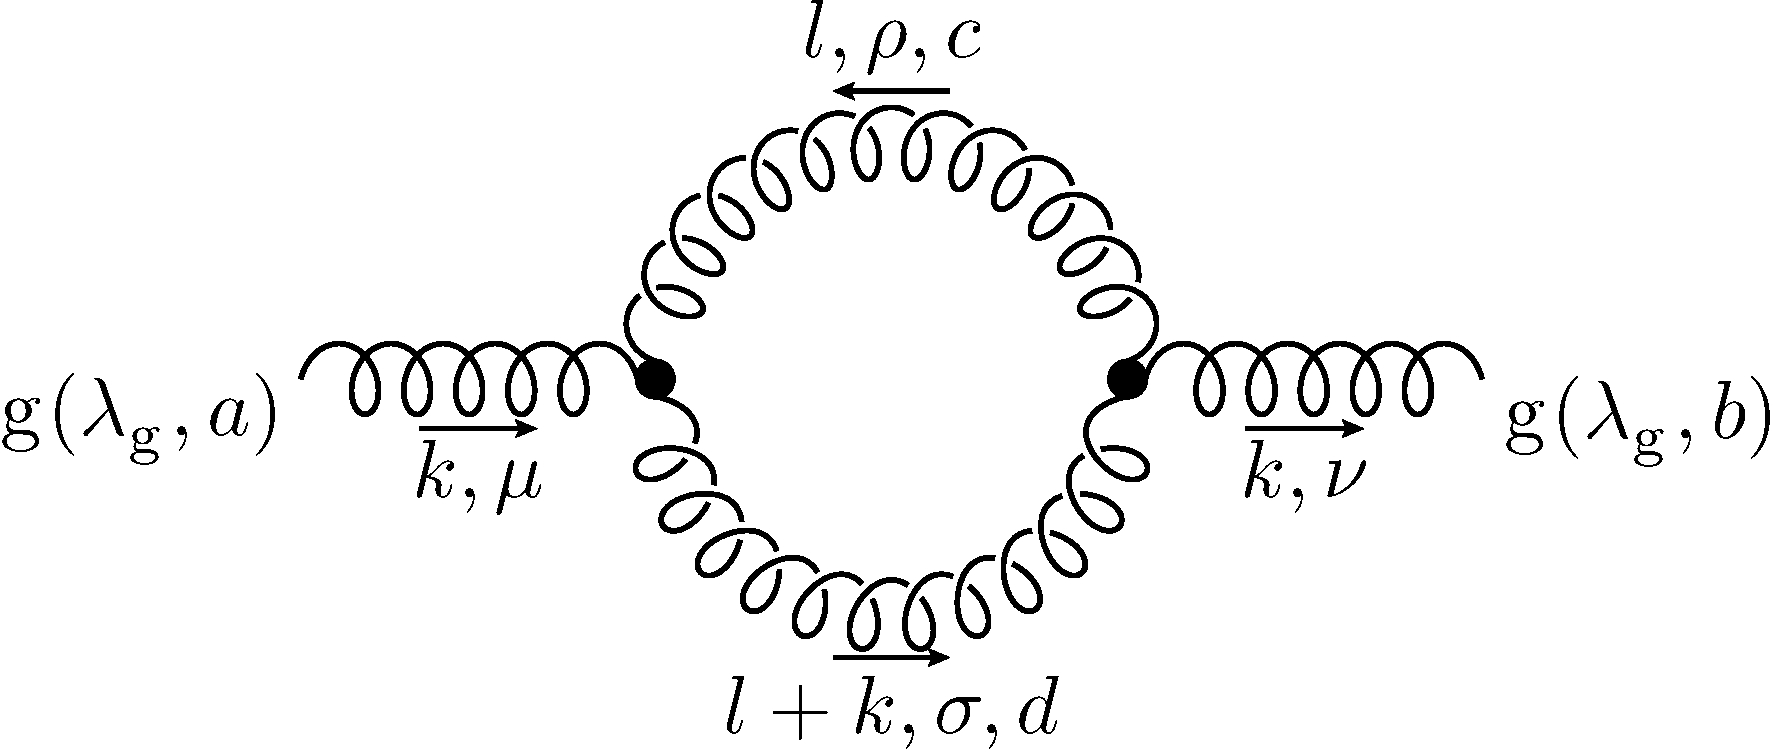
\includegraphics[width=\textwidth]{pyfeyn/nlo-v-seg}
		\caption{$-i\Pi_{\mu\nu}^{ab,(1)}(k)$}
	\end{subfigure}\hspace{.15\textwidth}%
	\begin{subfigure}[t]{.4\textwidth}
		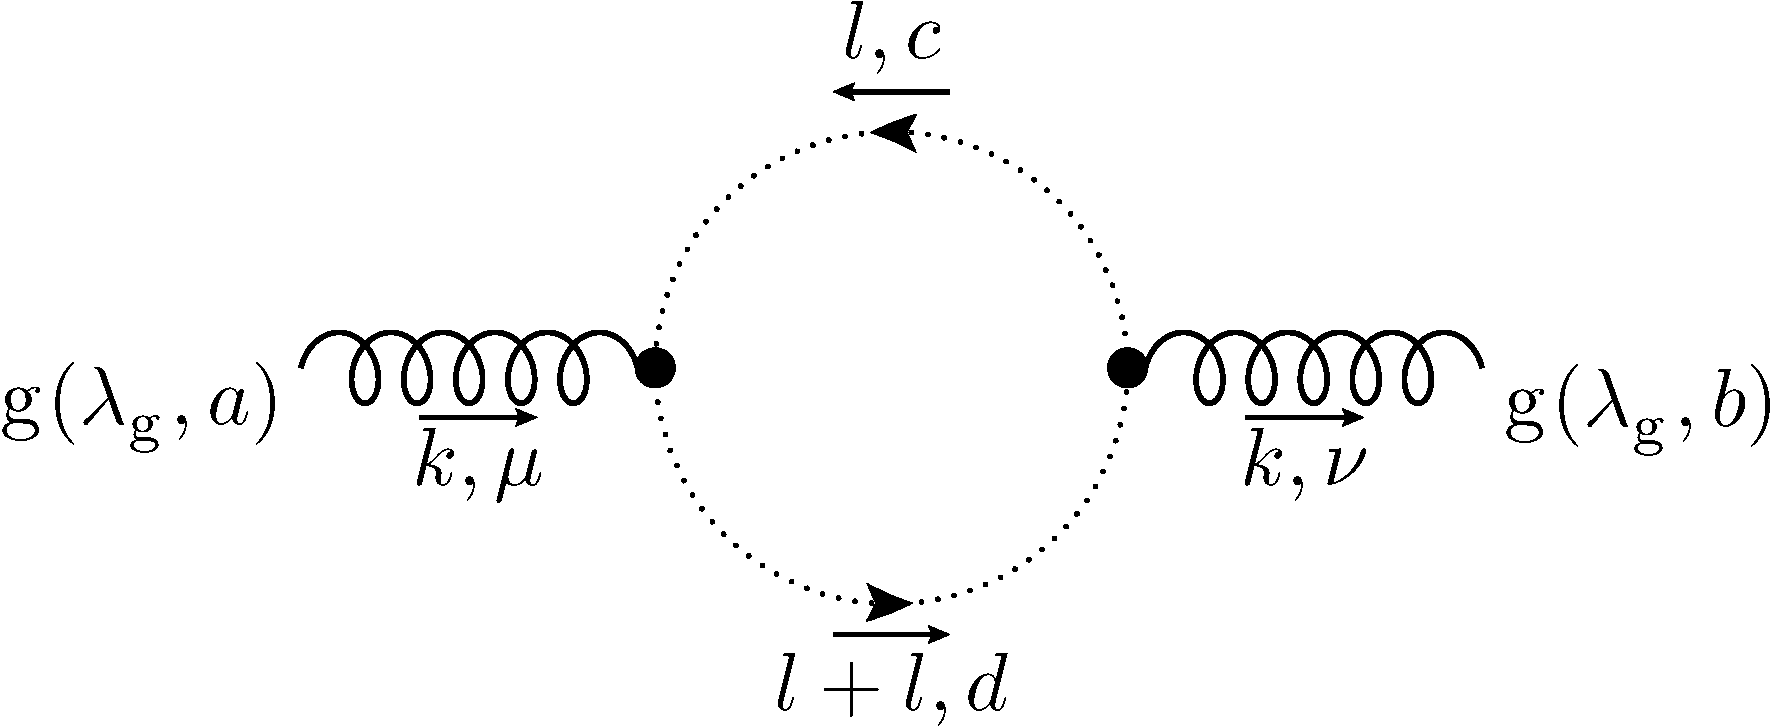
\includegraphics[width=\textwidth]{pyfeyn/nlo-v-seggh}
		\caption{$-i\Pi_{\mu\nu}^{ab,(2)}(k)$}
	\end{subfigure}\\
	\begin{subfigure}[t]{.4\textwidth}
		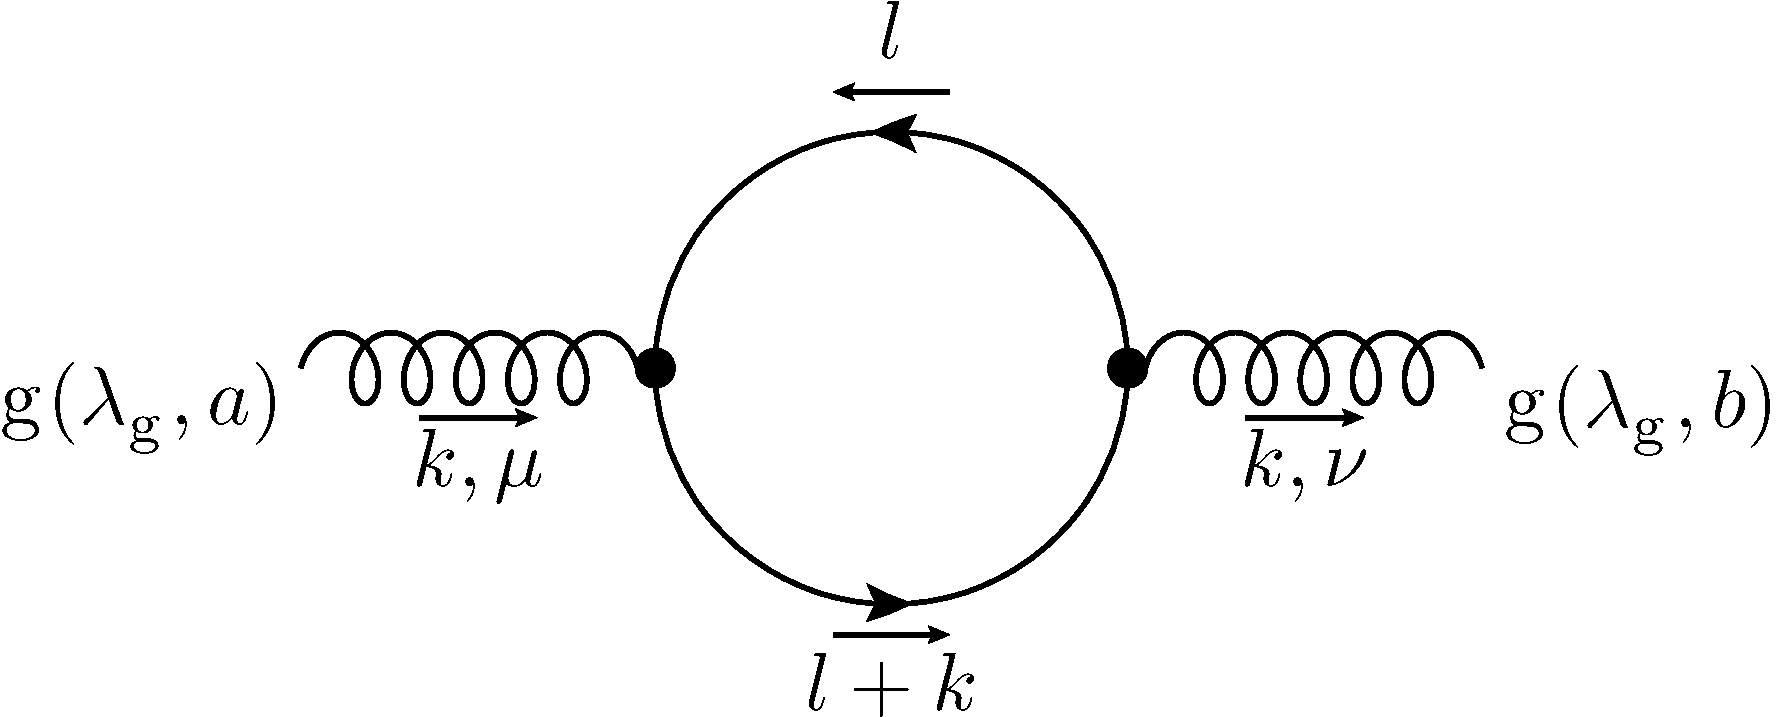
\includegraphics[width=\textwidth]{pyfeyn/nlo-v-segq}
		\caption{$-i\Pi_{\mu\nu}^{ab,(3)}(k)$}
	\end{subfigure}\hspace{.15\textwidth}%
	\begin{subfigure}[t]{.4\textwidth}
		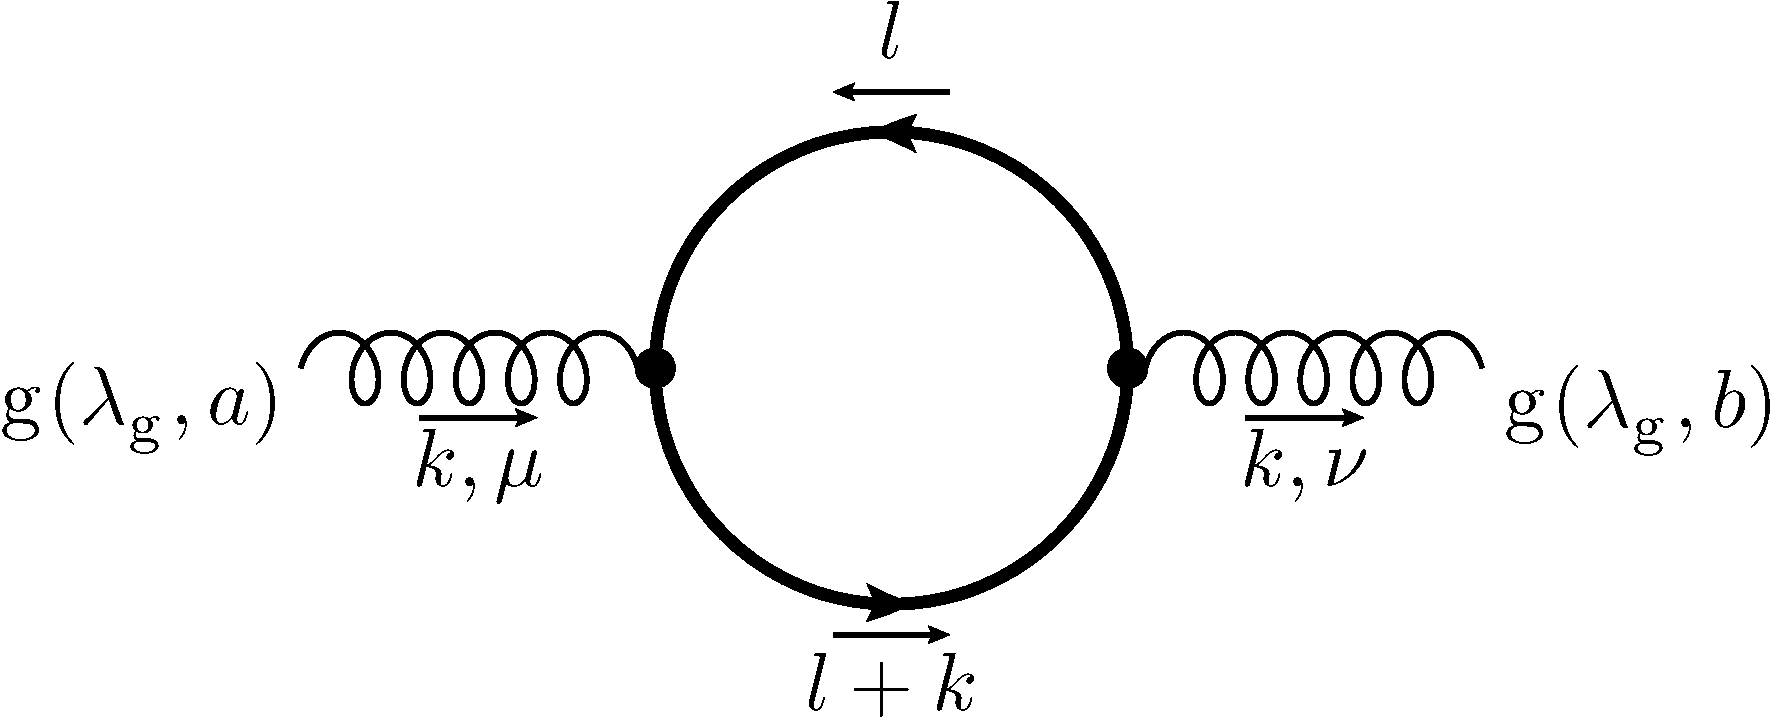
\includegraphics[width=\textwidth]{pyfeyn/nlo-v-seghq}
		\caption{$-i\Pi_{\mu\nu}^{ab,(4)}(k)$}
	\end{subfigure}\\
	\begin{subfigure}[t]{.4\textwidth}
		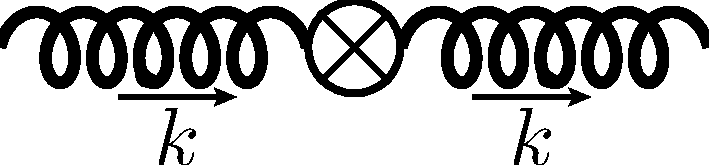
\includegraphics[width=\textwidth]{pyfeyn/nlo-v-segc}
		\caption{$-i\Pi_{\mu\nu}^{ab,(C)}(k)$}
	\end{subfigure}
	\caption{NLO contributions by quark self energy}\label{fig:FeynNLOvseqg}
\end{figure}

\begin{align}
-i\Pi_{\mu\nu}^{ab,(1)}(k) &= \frac 1 {2!} \mu_R^{4-n}\!\!\int\!\!\frac{d^nl}{(2\pi)^n} gf_{cda}\left(g_{\rho\sigma}(2l+k)_{\mu}+g_{\sigma\mu}(-l-2k)_\rho+g_{\mu\rho}(k-l)_\sigma\right)\nonumber\\
 &\hspace{30pt}\cdot gf_{cbd}\left(g^\rho_{\ \nu}(k-l)^\sigma+g_{\ \nu}^\sigma(-l-2k)^\rho+g^{\sigma\rho}(2l+k)_\nu\right)\cdot\frac{(-i)^2}{l^2(l+k)^2}\\
-i\Pi_{\mu\nu}^{ab,(2)}(k) &= -\mu_R^{4-n}\!\!\int\!\!\frac{d^nl}{(2\pi)^n} g^2 f_{adc}f_{bcd}l_\mu(l+k)_{\nu}\frac{i^2}{l^2(l+k)^2}\\
-i\Pi_{\mu\nu}^{ab,(3)}(k) &= -\mu_R^{4-n}\!\!\int\!\!\frac{d^nl}{(2\pi)^n} \frac{\tr\!\left((ig\gamma_\mu)(i\slashed l)\left(ig\gamma_\nu\right)(i(\slashed l + \slashed k))\right)\tr(T_aT_b)}{l^2(l+k)^2}\\
-i\Pi_{\mu\nu}^{ab,(4)}(k) &= -\mu_R^{4-n}\!\!\int\!\!\frac{d^nl}{(2\pi)^n} \frac{\tr\!\left((ig\gamma_\mu)(i(\slashed l + m))\left(ig\gamma_\nu\right)(i(\slashed l + \slashed k + m))\right)\tr(T_aT_b)}{(l^2-m^2)((l+k)^2-m^2)}\\
-i\Pi_{\mu\nu}^{ab,(C)}(k) &= i(Z_3-1)\delta^{ab}(k_\mu k_\nu-k^2g_{\mu\nu})
\end{align}

Color space:
\begin{align}
f_{acd}f_{bdc} &= -\delta_{ab} C_A = f_{dca}f_{dbc}\\
\tr(T_aT_b) &= \frac 1 2 \delta_{ab}
\end{align}

By Slavnov-Taylor\fxerror{cite} we know:
\begin{align}
\Pi_{\mu\nu}^{ab}(k) &= \delta^{ab}(k_\mu k_\nu-k^2g_{\mu\nu})\Pi(k^2)\\
\Rightarrow \Pi(k^2) &= -\frac{\delta_{ab}}{N_c^2-1}\frac 1 {(3+\epsilon)k^2}g^{\mu\nu}\Pi_{\mu\nu}^{ab}(k)
\end{align}

Gluon + Ghost loop:
\begin{align}
\Pi^{(1+2)}(k^2) &= -ig^2C_A\frac {1} {(3+\epsilon)k^2}\mu_R^{-\epsilon}\!\!\int\!\!\frac{d^nl}{(2\pi)^n} \frac{(8+3\epsilon)k\cdot l+(9+3\epsilon)k^2+(8+3\epsilon)l^2}{l^2(l+k)^2}\\
&= -ig^2C_A\frac {10+3\epsilon} {2(3+\epsilon)}\mu_R^{-\epsilon}\!\!\int\!\!\frac{d^nl}{(2\pi)^n} \frac{1}{l^2(l+k)^2}
\end{align}
with
\begin{align}
B_0(k^2,0,0) &= \mu_R^{-\epsilon}\!\!\int\!\!\frac{d^nl}{(2\pi)^n} \frac{1}{l^2(l+k)^2}\\
 &=\frac{i}{16\pi^2}\left(-\frac 2 {\hat\epsilon} -\ln(-k^2/\mu_R^2) + 2\right)
\end{align}
We find
\begin{align}
\Rightarrow \Pi^{(1+2)}(k^2) &= g^2C_A\left(-\frac {10} {3\hat\epsilon} - \frac 5 3\ln(-k^2/\mu_R^2) +\frac{31}{9}\right)\\
 &=-C_A\frac{g^2}{16\pi^2}\frac{5}{3}\left(\frac {2} {\hat\epsilon} + \ln(-k^2/\mu_R^2) -\frac{31}{15}\right)
\end{align}

Heavy quark loop:
\begin{align}
\Pi^{(4)}(k^2) &= ig^2\frac {1} {2(3+\epsilon)k^2}\mu_R^{-\epsilon}\!\!\int\!\!\frac{d^nl}{(2\pi)^n} \frac{4((2+\epsilon)(m^2-k\cdot l - l^2)+2m^2)}{(l^2-m^2)((l+k)^2-m^2)}\\
 &= ig^2\frac {2}{(3+\epsilon)k^2}\left(2m^2B_0(k^2,m^2,m^2)-(2+\epsilon)A_0(m^2)\right.\nonumber\\
 &\hspace{60pt}\left.-(2+\epsilon)k^2B_1(k^2,m^2,m^2)\right)
\end{align}
with
\begin{align}
A_0(m^2) &= \frac {i m^2}{16\pi^2}\left(-\frac 2 {\hat \epsilon_m} + 1 \right)\\
B_1(k^2,m^2,m^2) &= -\frac 1 2 B_0(k^2,m^2,m^2)\\
B_0(k^2,m^2,m^2) &= \frac i {16\pi^2}\left(-\frac 2 {\hat \epsilon_m} + 2 + \beta_k\ln(\chi_k) \right)
\end{align}
and $\beta_k=\sqrt{1-4m^2/k^2}$, $\chi_k=(\beta_k-1)/(1+\beta_k)$. We then find
\begin{align}
\Rightarrow \Pi^{(4)}(k^2) &= \frac {2g^2}{16\pi^2}\left(\frac 2 {3\hat \epsilon_m}-\frac 5 9 -\frac{4m^2}{3k^2} - \frac 1 3 \left(1+2\frac{m^2}{k^2}\right)\beta_k\ln(\chi_k)\right)\\
&= \frac {g^2}{16\pi^2}\frac 2 3\left(\frac 2 {\hat \epsilon_m}-\frac 5 3 -4\frac{m^2}{k^2} - \left(1+2\frac{m^2}{k^2}\right)\beta_k\ln(\chi_k)\right)
\end{align}

Light quark loop:
\begin{align}
\Pi^{(3)}(k^2) &= -ig^2\frac {2(2+\epsilon)}{(3+\epsilon)}B_1(k^2,0,0)\\
 &= ig^2\frac {(2+\epsilon)}{(3+\epsilon)}B_0(k^2,0,0)\\
 &=\frac{g^2}{16\pi^2}\frac 2 3\left(\frac 2 {\hat \epsilon} + \ln(-k^2/\mu_R^2)-\frac 5 3\right)
\end{align}

We choose the counterterm to be:
\begin{align}
-\Pi^{(C)}(k^2)=Z_3-1 &= \frac{g^2}{16\pi^2}\left(-\frac 5 3 C_A \frac 2 {\hat \epsilon} + n_{lf}\frac 2 3 \frac 2 {\hat \epsilon} + \frac 2 3 \frac 2 {\hat \epsilon_m}\right)\\
 &= \frac{g^2}{16\pi^2}\left( (2C_A-\beta_0^{lf})\frac 2 {\hat\epsilon}+ \frac 2 3 \frac 2 {\hat \epsilon_m} \right)\\
 &= \frac{g^2}{16\pi^2}\left( (2C_A-\beta_0^f)\frac 2 {\hat\epsilon}+ \frac 2 3 \ln(m^2/\mu_R^2) \right)
\end{align}
with $\beta_0^{lf} = (11C_A-2n_{lf})/3$, $\beta_0^f = (11C_A-2n_{f})/3$ and $n_f=n_{lf}+1$.

We also find
\begin{equation}
Z_g -1 = \frac{g^2}{16\pi^2}\frac 1 2\left(\beta_0^f\frac 2 {\hat\epsilon} - \frac 2 3 \ln(m^2/\mu_R^2) \right)
\end{equation}
such that $g\rightarrow Z_g g$.


\subsubsection{Gluon Self Energy (On shell)}
We have\cite[(A.18)-(A.20)]{Pokorski}:
\begin{align}
I_0 &= \int\!\frac{d^np}{(2\pi)^n} \frac 1 {(p^2+2kp+M^2+i\eta)^\alpha}\\
 &= i\frac{(-\pi)^{n/2}}{(2\pi)^n} \frac{\Gamma(\alpha-n/2)}{\Gamma(\alpha)} \frac 1 {(M^2-k^2+i\eta)^{\alpha-n/2}}\\
I_\mu &= \int\!\frac{d^np}{(2\pi)^n} \frac {p_\mu} {(p^2+2kp+M^2+i\eta)^\alpha}\\
 &= - k_\mu I_0\\
I_{\mu\nu}&= \int\!\frac{d^np}{(2\pi)^n} \frac {p_\mu p_\nu} {(p^2+2kp+M^2+i\eta)^\alpha}\\
 &= I_0\left(k_\mu k_\nu + \frac 1 2 g_{\mu\nu}(M^2-k^2)\frac 1 {\alpha-n/2-1}\right)
\end{align}

Heavy Quark loop:
\begin{align}
-i\Pi_{\mu\nu}^{ab,(4)}(k) &=  -\mu_R^{4-n}\!\!\int\!\!\frac{d^nl}{(2\pi)^n} \frac{\tr\!\left((ig\gamma_\mu)(i(\slashed l + m))\left(ig\gamma_\nu\right)(i(\slashed l + \slashed k + m))\right)\tr(T_aT_b)}{(l^2-m^2)((l+k)^2-m^2)}\\
 &= -\frac {\delta^{ab}}{2}g^2\mu_R^{4-n}\!\int\limits_0^1dx\!\!\int\!\!\frac{d^nl}{(2\pi)^n} 4\frac{2l_\mu l_\nu+(l_\mu k_\nu+l_\nu k_\mu)+(m^2-k\cdot l-l^2)g_{\mu\nu}}{(l^2+2xk\cdot l-m^2+k^2 x)^2}\\
 &= -2\delta^{ab}g^2\mu_R^{4-n}\!\int\limits_0^1dx\!\left(2I_{\mu\nu}+\left(k_\nu I_\nu + k_\nu I_\mu\right) + g_{\mu\nu}\left(m^2I_0-k^\rho I_\rho - g_\rho^{\,\sigma}I_{\rho\sigma}\right)\right)\\
 &= -2\delta^{ab}g^2\mu_R^{4-n}\!\!\int\limits_0^1dx\,I_0\left[k_\mu k_\nu(2x^2-2x)+\right.\nonumber\\
 &\hspace{60pt}\left.g_{\mu\nu}\left((k^2x(1-x)-m^2)\frac{1-n/2}{1-n/2}+m^2+k^2x(1-x)\right)\right]\\
 &= 4\delta^{ab}g^2(k_\mu k_\nu - g_{\mu\nu}k^2) \mu_R^{4-n}\!\!\int\limits_0^1\!dx\,x(1-x)I_0
\end{align}
where
\begin{align}
\mu_R^{4-n}I_0 &= i\frac{(-\pi)^{n/2}}{(2\pi)^n} \frac{\Gamma(2-n/2)}{\Gamma(2)} \left(\frac {\mu_R^2} {k^2x(1-x)-m^2}\right)^{2-n/2}\\
 &= -\frac i {16\pi^2}\left(\frac 2 {\hat\epsilon}-\ln((k^2x(1-x)-m^2)/\mu_R^2)\right) + O(\epsilon)
\end{align}
so for $k^2=0$ (on shell) we end up with
\begin{equation}
-i\Pi_{\mu\nu}^{ab,(4)}(k) = -i\delta^{ab}\frac{g^2}{16\pi^2}(k_\mu k_\nu - g_{\mu\nu}k^2) \frac 4 {3\hat\epsilon_m}
\end{equation}

Light Quark loop:
\begin{align}
-i\Pi_{\mu\nu}^{ab,(3)}(k) &= -\mu_R^{4-n}\!\!\int\!\!\frac{d^nl}{(2\pi)^n} \frac{\tr\!\left((ig\gamma_\mu)(i\slashed l)\left(ig\gamma_\nu\right)(i(\slashed l + \slashed k))\right)\tr(T_aT_b)}{l^2(l+k)^2}\\
 &= 4\delta^{ab}g^2(k_\mu k_\nu - g_{\mu\nu}k^2) \mu_R^{4-n}\!\!\int\limits_0^1\!dx\,x(1-x)I_0
\end{align}
where
\begin{align}
\mu_R^{4-n}I_0 &= \mu_R^{4-n}\!\!\int\!\!\frac{d^nl}{(2\pi)^n} \frac 1 {(l^2+2xk\cdot l+k^2x)^2}\\
 &= \mu_R^{4-n}\!\!\int\!\!\frac{d^nl}{(2\pi)^n} \frac 1 {((l+xk)^2+k^2x(1-x))^2}
\end{align}
so for $k^2=0$ (on shell) we get $I_0 = 0$ and end up with
\begin{equation}
-i\Pi_{\mu\nu}^{ab,(3)}(k) = 0
\end{equation}

Gluon + Ghost loop vanish by the same arguments as the light quark loop:
\begin{equation}
-i\Pi_{\mu\nu}^{ab,(1+2)}(k) = 0
\end{equation}

